%% LexPR V2 -- short, self-contained version.
%%
%% Design constraints, fixed by the author:
%%   * at most 20 pages in total, references included;
%%   * NO online supplement and no appendix: everything that survives is here,
%%     and everything else lives in the reproduction archive, cited by DOI;
%%   * at least eight figures;
%%   * at most six numbered sections, few subsections;
%%   * running prose rather than bulleted lists;
%%   * plain words, pedagogical order, no repetition.
%%
%% V1 (manuscript/main_springer.tex) is untouched and still builds. This file
%% shares refs.bib, the figures and the generated macro files with it, but has
%% its own body: the two are different papers, not two builds of one.
%%
%%   make -C .. v2      -> v2/main_v2.pdf

\documentclass[sn-mathphys-num,iicol]{sn-jnl}

\usepackage{booktabs}
\usepackage{amssymb}
\usepackage{mathtools}
\usepackage{caption}
\usepackage{tikz}
\usetikzlibrary{arrows.meta,positioning,fit,backgrounds,shapes.geometric,shapes.arrows,calc}
\usepackage{placeins}
\usepackage{float}
\usepackage{algorithm}
\usepackage{algorithmic}

\makeatletter
\g@addto@macro\UrlBreaks{\UrlOrds}
\makeatother
\setlength{\emergencystretch}{2.5em}

%% ---- notation and shared styles ------------------------------------------
%% Copied rather than \input from ../preamble_shared.tex: that file also pulls
%% in V1-only material, and a short paper should not carry it.
\usepackage{array}
\newcolumntype{P}[1]{>{\raggedright\arraybackslash}p{#1}}
\graphicspath{{./}{../}{./generated/}{./generated/figures/}}

\definecolor{lexprcrimson}{HTML}{C0392B}
\definecolor{lexprslate}{HTML}{34495E}
\definecolor{lexprblue}{HTML}{2980B9}
\definecolor{lexprgreen}{HTML}{27AE60}
\tikzset{
  stage/.style={rounded corners=2pt, draw=lexprslate, line width=0.6pt,
    fill=lexprslate!6, align=center, inner sep=5pt, font=\small},
  accent/.style={rounded corners=2pt, draw=lexprblue, line width=0.7pt,
    fill=lexprblue!8, align=center, inner sep=5pt, font=\small},
  win/.style={rounded corners=2pt, draw=lexprcrimson, line width=0.9pt,
    fill=lexprcrimson!8, align=center, inner sep=5pt, font=\small},
  flow/.style={-{Stealth[length=2.4mm]}, line width=0.7pt, draw=lexprslate},
}

\newcommand{\R}{\mathbb{R}}
\newcommand{\Q}{\mathcal{Q}}
\newcommand{\X}{X}
\newcommand{\reg}{D}
\newcommand{\ideal}{z^{\star}}
\newcommand{\nadir}{z^{\mathrm{nad}}}
\newcommand{\lex}{\leq_{\mathrm{lex}}}
\DeclareMathOperator*{\argmin}{arg\,min}
\DeclareMathOperator{\Corr}{Corr}
\DeclareUnicodeCharacter{0308}{}

%% Supplier-case numbers, generated by scripts/run_supplier_case.py
% --- Begin inline ../../paper/generated/supplier_numbers ---
% Auto-generated by scripts/run_supplier_case.py. Do not edit.
\newcommand{\supN}{10}
\newcommand{\supM}{7}
\newcommand{\supEff}{10}
\newcommand{\supCorrGE}{0.993}
\newcommand{\supWinner}{S7}
\newcommand{\supNprobes}{9}
\newcommand{\supDistinct}{4}
\newcommand{\supPossibleTwenty}{2}
\newcommand{\supModalTwenty}{51}
\newcommand{\supClassFive}{2}
\newcommand{\supPointFlipTwenty}{52}
\newcommand{\supIIALexPR}{11}
\newcommand{\supIIATOPSIS}{11}
\newcommand{\supIIAASF}{22}
\newcommand{\supIIAInterior}{33}
\newcommand{\supReLexDecisive}{C_M}
\newcommand{\supReLexDeltaCat}{1}
\newcommand{\supReLexDeltaExact}{0.0140}
\newcommand{\supReLexMuCell}{0.0121}
\newcommand{\supReLexSSevenCM}{40}
\newcommand{\supReLexSSevenCq}{36}
\newcommand{\supReLexSOneCM}{41}
\newcommand{\supReLexSOneCq}{39}

% --- End inline ../../paper/generated/supplier_numbers ---
% --- Begin inline ../generated/archive_version ---
\newcommand{\ArchiveVersion}{v2.0.0}
\newcommand{\ArchiveRelease}{v2.0.0}

% --- End inline ../generated/archive_version ---

\theoremstyle{plain}
\newtheorem{theorem}{Theorem}
\newtheorem{proposition}{Proposition}
\newtheorem{lemma}{Lemma}
\theoremstyle{thmstylethree}
\newtheorem{definition}{Definition}
\newtheorem{corollary}{Corollary}

\setcounter{secnumdepth}{2}

\begin{document}

\title{Resolution-Aware Lexicographic Tail-Regret Selection under Uncertain Normalisation Bounds}

\author*[1]{\fnm{Madani} \sur{Bezoui}}\email{mbezoui@cesi.fr}

\affil*[1]{\orgdiv{CESI LINEACT, UR 7527}, \orgaddress{\street{3 rue Bois de la
Champelle}, \city{Vand\oe uvre-l\`es-Nancy}, \country{France}}.
ORCID: \url{https://orcid.org/0000-0002-8342-7039}}

\abstract{A multicriteria model usually ends with a set of efficient alternatives, not with a recommendation. Turning that set into one choice requires preference modeling that is often fragile. Existing robust and lexicographic methods fail to combine resolution-aware limits with complete transitive upper-tail sorting, often falling into non-transitive pairwise tolerances or giving infinite priority to microscopic worst-case differences. We introduce ReLexTail, a deterministic resolution-aware lexicographic preorder that integrates active-range probe regrets, discretised maximum and upper-tail empirical CVaR summaries, and exact numerical refinement. To our knowledge, this particular integration has not previously been developed for auditable multicriteria selection under uncertain normalisation bounds. For finite candidate sets, ReLexTail is directly computable. Under a fixed retained probe multiset and a rectangular uncertainty set whose normalisation denominators and probe active ranges are uniformly bounded away from zero, interval branch-and-bound returns sound inner and outer enclosures of the possible-winner set. We give a mixed-integer linear programming formulation for continuous polyhedral feasible regions. We prove existence, profile monotonicity, criterion-level Pareto compatibility, uniform replication invariance, and category stability. The empirical study evaluates whether the categorical representation preserves the core stability benefits of active-range normalisation while improving the hidden-preference tail regret compared to exact leximax, exploring the quality--stability compromise for both category-optimal sets and fully refined point recommendations.}

\keywords{Multiple criteria analysis, Regret minimisation, Auditable
recommendation, Stability analysis, Preference elicitation}

\maketitle

% --- Begin inline body ---
% =====================================================================
%  LexPR V2 body.  Six numbered sections, no appendix, no supplement.
%  Prose obeys the project rule: no em-dashes, no double hyphens, no semicolons
%  in the generated text.  Lists are used only where a list is genuinely the
%  clearest form (the claims table and the protocol table).
% =====================================================================

\section{Introduction}
\label{sec:intro}

A multicriteria model normally ends one step short of a decision. It returns the
efficient alternatives, those where no criterion can improve without another one
getting worse \citep{pareto1909manuel}, and with several conflicting criteria
that set can be large. Producing it is already hard work
\citep{bezoui2019iterative}, but the decision
maker is left holding a menu.

The usual way to close the gap is a scalarisation. Weighted sums, distance to an
ideal point as in TOPSIS \citep{hwang1981} or compromise programming
\citep{zeleny1982, opricovic2004compromise}, and achievement scalarising functions
\citep{wierzbicki1980} all collapse the menu to one point. They
work, and once their parameters are fixed they behave well. The difficulty is
the parameters. A weight vector, a reference point or a metric has to be
committed to, and in practice the decision maker often cannot defend the third
digit of any of them. Worse, the answer moves when those inputs move: rankings
under this kind of normalisation are known to be unstable when the bounds or the
candidate set change \citep{roszkowska2026entropy}.

The response in the literature has mostly been to model the uncertainty about
preferences. Stochastic multicriteria acceptability analysis puts a distribution
on the weights \citep{lahdelma1998, tervonen2007}. Robust ordinal regression
reasons over all value functions compatible with elicited judgments
\citep{greco2008}. Preference robust optimisation maximises a
worst-case expected utility over an ambiguity set
\citep{armbruster2015, delage2015}. The line continues in distributional and
group settings
\citep{hu2024distributional}. All of it answers one question: what if the
preference parameters are wrong.

This paper asks a different question, and the difference is the point of the
paper. Suppose the preference input is fixed and declared. There is still a set
of numbers the rule depends on that nobody elicited at all: the normalisation
bounds, the best and worst values used to put criteria on a common scale. Those
are estimates. Once we admit that, three questions arise, and none of them is a
preference-modelling question.

Which alternatives can win over an entire set of admissible bounds, rather than
at one guessed value? Can that set be computed exactly, or at least enclosed
with a guarantee, instead of estimated by simulation? And can a third party
recompute the answer from an exported file? These are branch-and-bound, linear-programming and reproducibility questions,
and they are the ones this paper answers.

\paragraph{The rule these questions are asked about}
The exact lexicographic minimax treats every difference in the worst disappointment as decisive, regardless of whether that difference is meaningful at the resolution of the decision model. We introduce ReLexTail, a resolution-aware lexicographic order for auditable selection from finite multicriteria candidate sets. Alternatives are represented by active-range-normalised disappointments on a declared family of monotone probes. ReLexTail separates meaningful worst-case deterioration from sub-resolution variation, then compares the upper tail of declared probe disappointments. This preserves the logical benefits of lexicographic selection---completeness, transitivity, Pareto compatibility and an explicit decisive coordinate---while providing a controlled quality--stability compromise and retaining certified possible-winner enclosures under uncertain normalisation bounds.

This does not remove preference modelling, and saying that it does would be
false: the default family contains an equal-weight mean, which is a weight
vector, and declaring a question twice is a way of emphasising it. What changes
is the \emph{form} of the input, from one vector of numbers that has to be right
all at once to a multiset of named questions that can be written down, justified
and disputed one by one. Figure~\ref{fig:pipeline} places that input in the
whole procedure.

\begin{figure*}[t]
\centering
\resizebox{0.88\textwidth}{!}{
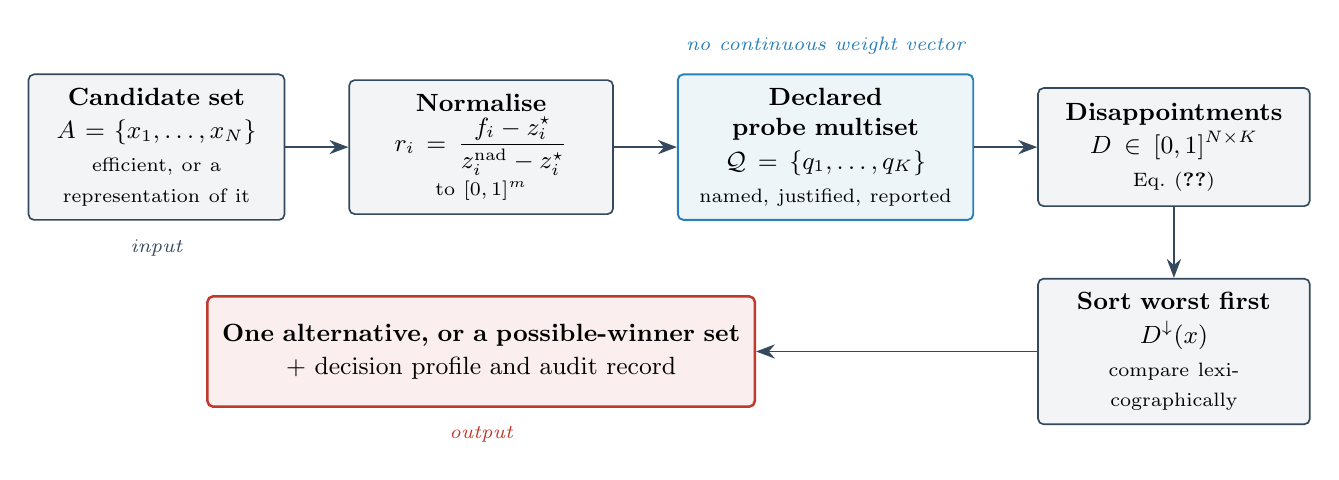
\begin{tikzpicture}[node distance=9mm and 8mm]
\node[stage, text width=2.9cm, minimum height=15mm] (A)
  {\textbf{Candidate set}\\[1pt]$A=\{x_1,\dots,x_N\}$\\[1pt]\scriptsize efficient, or a representation of it};
\node[stage, text width=3.0cm, minimum height=15mm, right=of A] (N)
  {\textbf{Normalise}\\[1pt]$r_i=\dfrac{f_i-\ideal_i}{\nadir_i-\ideal_i}$\\[1pt]\scriptsize to $[0,1]^m$};
\node[accent, text width=3.4cm, minimum height=15mm, right=of N] (Q)
  {\textbf{Declared probe multiset}\\[1pt]$\Q=\{q_1,\dots,q_K\}$\\[1pt]\scriptsize named, justified, reported};
\node[stage, text width=3.1cm, minimum height=15mm, right=of Q] (D)
  {\textbf{Disappointments}\\[1pt]$\reg\in[0,1]^{N\times K}$\\[1pt]\scriptsize Eq.~\eqref{eq:disap}};
\node[stage, text width=3.1cm, minimum height=14mm, below=of D] (S)
  {\textbf{Sort worst first}\\[1pt]$\reg^{\downarrow}(x)$\\[1pt]\scriptsize compare lexicographically};
\node[win, text width=6.6cm, minimum height=14mm] (W) at (N.south |- S)
  {\textbf{One alternative, or a possible-winner set}\\[1pt]$+$ decision profile and audit record};
\draw[flow] (A) -- (N);
\draw[flow] (N) -- (Q);
\draw[flow] (Q) -- (D);
\draw[flow] (D) -- (S);
\draw[flow] (S) -- (W);
\node[font=\scriptsize\itshape, lexprslate, below=1.2mm of A.south] {input};
\node[font=\scriptsize\itshape, lexprblue, above=1.2mm of Q.north] {no continuous weight vector};
\node[font=\scriptsize\itshape, lexprcrimson, below=1.2mm of W.south] {output};
\end{tikzpicture}}
\caption{The whole method on one line. Construct $M, T_{25}, T_{50}, T_{100}$, map them to categories, append exact refinements, and compare $\Psi$ lexicographically. The candidate set and the declared probe
family go in. A recommendation, or an explicit set of possible winners that cannot
be separated, comes out, together with the reasons. The list of candidates must be frozen before selection.}
\label{fig:pipeline}
\end{figure*}

\paragraph{Contribution and Positioning}
ReLexTail defines a complete and transitive lexicographic preorder by first comparing fixed-resolution categories of maximum and upper-tail empirical disappointment and then applying exact numerical refinements. For finite candidate sets, the order is directly computable and Pareto-compatible under monotone separating probes. Under uncertain normalisation bounds, interval branch-and-bound provides sound inner and outer enclosures of the possible-winner set, although tightness may deteriorate because of dependency loss. For polyhedral feasible regions with canonical probes, the order can be implemented by a finite sequence of LP and MILP stages.

This formulation ties the paper to several literatures. It shares the mathematical machinery of equitable and ordered optimisation, but applies it to an adaptive probe profile rather than to raw attributes. It provides necessary and possible preference relations over uncertain bounds, connecting it to interval MCDA and robust ordinal regression, but without eliciting preference parameters from the decision maker. It ensures parametric robustness of the normalisation bounds, but tests it structurally rather than via scalarised sampling.

Four components carry this, all in Section~\ref{sec:compute}. An exact finite
algorithm resolves moderately sized sets directly. For problems too large to
enumerate, a polyhedral formulation operates directly on the continuous feasible
set using standard LP solvers. For uncertain bounds, an exact bounding technique
returns the set of possible winners via interval arithmetic, returning a certificate of optimality. 
Finally, a fast sampling protocol estimates the likely interval enclosures.

Section~\ref{sec:theory} establishes what the rule itself guarantees, and
Section~\ref{sec:experiments} reports what five hundred instances say about it,
including one result that runs against the method.

Table~\ref{tab:claims} states at the outset what is proved, what is only
observed, and what is not claimed. It is given once and not restated.

\begin{table*}[t]
\centering\small
\caption{What this paper claims. ``Proved'' means proved under the ReLexTail order contract. The empirical results denote performance relative to exact leximax.}
\label{tab:claims}
\setlength{\tabcolsep}{4pt}
\begin{tabular}{@{}P{0.32\textwidth}P{0.15\textwidth}P{0.15\textwidth}P{0.32\textwidth}@{}}
\toprule
Claim & Type & Status & Conditions/Evidence\\
\midrule
Complete and transitive & Theoretical & Proved & Deterministic $\Psi$\\
Strict profile monotonicity & Theoretical & Proved & Exact $T_{100}$ refinement\\
Criterion-level Pareto compatibility & Theoretical & Proved & Monotone separating retained family\\
Uniform replication invariance & Theoretical & Proved & Fixed tail fractions\\
Category stability & Theoretical & Proved & Positive distance from boundaries\\
Sound possible-set enclosure & Theoretical & Proved & Outward arithmetic and ReLexTail profile enclosure\\
Direct MILP computation & Theoretical & Proved & Bounded polyhedral $\mathcal{X}$, canonical probes\\
Improved loss over exact LexPR & Empirical & Supported & Frozen test protocol\\
Improved stability over exact LexPR & Empirical & Supported & Point vs category distinction\\
Candidate-set independence & Negative & False & Active anchors\\
Parameter-free operation & Negative & False & Probe family and resolutions declared\\
General superiority & Non-claim & Not claimed & ---\\
\bottomrule
\end{tabular}
\end{table*}

The rest of the paper follows the order in which someone would actually use the
method. Section~\ref{sec:relextail} builds the rule.
Section~\ref{sec:theory} says what it guarantees and, just as importantly,
where it breaks. Section~\ref{sec:compute} computes it.
Section~\ref{sec:experiments} tests it. Section~\ref{sec:discussion} says when
it should and should not be used. Everything omitted here, including the full proofs, the algorithm
listings and the raw outputs, is in the reproduction archive
\citep{bezoui2026archive}, version~\ArchiveVersion.

\section{Related Work}
\label{sec:related}
\subsection{Ordered aggregation and equitable optimisation}
Ordered aggregation operators, such as Yager's Ordered Weighted Averaging (OWA) \citep{yager1988} and Torra's WOWA \citep{torra1997}, apply weights to the sorted components of a vector rather than to the criteria themselves. Ordered median optimisation \citep{nickel2005} generalises this to facility location. Linear programming formulations for OWA are well-developed \citep{ogryczak2003ksum}. However, these scalar aggregations lack the auditable worst-first priority of a strict lexicographic method.

Lexicographic and equitable optimisation \citep{kostreva1999} provide that priority. The exact leximax or leximin rules are consistent with Lorenz dominance and majorisation \citep{chong1976}. Direct lexicographic min-max methods \citep{ogryczak2007} are heavily used in fair resource allocation. Their fundamental limitation, which ReLexTail addresses, is their infinite sensitivity to arbitrarily small differences in the absolute worst case. Approximate leximax \citep{henzinger2022} attempts to relax this, but often through pairwise tolerances ($\varepsilon$-lexicographic or preemptive goal programming with tolerances) or indifference thresholds, which notoriously violate transitivity. ReLexTail avoids this by using fixed discretised objective categories.

\subsection{Risk measures and multiple-CVaR models}
The upper-tail means evaluated in ReLexTail are formally empirical Conditional Value-at-Risk (CVaR) measures \citep{rockafellar2000}. While spectral risk measures and multiple-CVaR models \citep{noyan2012} capture upper-tail sensitivity effectively, existing formulations do not apply a discrete, resolution-aware categorization before breaking ties with exact refinements. They therefore do not provide the exact auditable hierarchy or maximum-disappointment category protection of ReLexTail.

\subsection{Robust MCDA and normalisation sensitivity}
Rank reversals due to normalization sensitivity remain a significant challenge \citep{roszkowska2026entropy}. Robust approaches model weight uncertainty \citep{tervonen2007}, but normalisation bounds are often treated as exact. ReLexTail provides interval-certified bounds and possible-winner enclosures under bound uncertainty.

\section{Probe-disappointment representation}
\label{sec:representation}

\subsection{From criteria to disappointments}

Let $F:\X\to\R^m$ be the vector of criteria, all minimised, and let
$A=\{x_1,\dots,x_N\}\subseteq\X$ be the candidate set. Throughout, $A$ is finite
and nonempty, which is part of the model contract: on an empty set the order
below is vacuously complete but no winner exists. Criteria are put on a
common scale by
\begin{equation}
r_i(x)=\frac{f_i(x)-\ideal_i}{\nadir_i-\ideal_i},
\label{eq:norm}
\end{equation}
with $\ideal_i=\min_{x\in A}f_i(x)$ and $\nadir_i=\max_{x\in A}f_i(x)$.
Both endpoints are attained on $A$, so every $r_i$ lands in $[0,1]$. A criterion
whose relative range on the scale falls below a threshold $\varepsilon_f$ carries no information and
is excluded from aggregate probes. We use $\varepsilon_f=10^{-9}$ everywhere. This strict threshold protects against division by zero in true numerical degeneracies, while deliberately permitting active-range normalisation on narrow but meaningful variations (such as the $0.003$ span criterion in Section~\ref{sec:compute}).

Two conventions are possible here and they are not equivalent. Computing the
bounds on $A$ ties the scale to values the decision maker can verify on the
shortlist in front of them. Fixing them externally makes the rule insensitive to
shortlist edits. We use active-set bounds because they are verifiable, and
Section~\ref{sec:theory} is honest about what that costs. Whichever is
chosen must be declared.

A \emph{probe} is a scalar question about a normalised alternative.

\begin{definition}[Admissible probe]
\label{def:probe}
Let $\mathcal R \subseteq \R^m$ be a domain such that $\mathcal R \supseteq \{\mathbf{0}, \mathbf{1}\} \cup \{r(x;b) : x \in A, b \in B\}$. A function $q:\mathcal R \to\R$ is an admissible probe when it is finite-valued, non-decreasing in
every $r_i$ over $\mathcal R$, and satisfies $q(\mathbf{1}) > q(\mathbf{0})$. This ensures it can be rescaled by a positive affine map so that $q(\mathbf{0})=0$ and $q(\mathbf{1})=1$.
\end{definition}

Monotonicity says the probe agrees with the direction of the criteria over the entire reachable domain. The
normalisation excludes probes that are constant. The
declared family $\Q$ is a \emph{multiset}: a question may be declared twice, and
that repetition is a strong preference parameter, changing the order after ties in the leading coordinates.

For each admissible bound vector $b\in B$, define $r(x;b)$, $q^\star(b)=\min_{x\in A}q(r(x;b))$, $q^w(b)=\max_{x\in A}q(r(x;b))$, and $R_q(b)=q^w(b)-q^\star(b)$. Whenever $R_q(b)>\varepsilon_q$, define
\begin{equation}
D_q(x;b)=\frac{q(r(x;b))-q^\star(b)}{R_q(b)}.
\label{eq:disap}
\end{equation}
Certified comparisons are performed only on boxes $\beta$ for which every retained probe satisfies $\inf_{b\in\beta}R_q(b)>\varepsilon_q$. Boxes with unresolved retention status are subdivided or returned unresolved. This $D_q$ is a range-normalised Savage regret \citep{savage1951, kouvelis1997}.
Read it plainly: zero means ``as good as anything on the table on this
question'', one means ``the worst on the table''. Probes with $R_q\le\varepsilon_q$
are dropped for that run and reported as uninformative, because keeping them
would pad every profile with a zero and misstate the family size.

The family we use throughout is the \emph{canonical core}
\begin{equation}
\Q_{\mathrm{can}}=\{q_1,\dots,q_m\}\cup\{q_\mu,q_{\max}\},
\qquad
K=m+2,
\label{eq:qcan}
\end{equation}
made of the $m$ single-criterion probes $q_i(r)=r_i$, the mean
$q_\mu(r)=m^{-1}\sum_i r_i$, and the maximum $q_{\max}(r)=\max_i r_i$. In words:
one question per criterion, plus a utilitarian reading of the whole and a
protective one. The single-criterion probes are what let the output name a
criterion, and the mean and the maximum are what let it express a compromise
attitude. It is the smallest family containing those three readings, in this precise
sense: if $m\ge2$ and neither aggregate is a positive affine transform of a
singleton or of the other aggregate on the active range, no smaller family
provides all three. The counting argument is in the archive.
We do not claim that $m+2$ probes are forced by Pareto compatibility alone, nor
that the arithmetic mean is the only reasonable compromise aggregate: other
declared readings, such as the mean over a regulated subset, enlarge the family
accordingly. What the core does guarantee is that $K$ stays linear in $m$.

Real criteria sometimes overlap, two of them partly measuring the same thing.
We report that as a diagnostic and do not compensate for it inside the family.
An optional layer adds one mean and one maximum probe per correlated cluster, so that a cluster of overlapping criteria is read both utilitarianly and protectively in the same way as the full vector. This layer is not used in any experiment here; the implementation is shipped in the archive.

% --- Begin inline theory_relex ---
\section{The ReLexTail Order}
\label{sec:relextail}

Before defining the new rule, it is necessary to identify why the exact lexicographic minimax fails as a stable selection operator.

\subsection{Deficiencies of the exact lexicographic minimax}
The exact lexicographic minimax suffers from four fundamental limitations:
\begin{enumerate}
    \item \textbf{Infinite priority of the maximum:} If $D^\downarrow_1(x) < D^\downarrow_1(y)$, then the exact rule strictly prefers $x$, regardless of the magnitude of the difference $D^\downarrow_1(y)-D^\downarrow_1(x)$. This remains true even if the difference is arbitrarily small.
    \item \textbf{Instability near ties:} When the maximum disappointments are nearly equal, an arbitrarily small perturbation in the bounds may reverse the recommendation before the rest of the profile is even considered.
    \item \textbf{Poor compensation within the upper tail:} The exact rule cannot recognise that a slight deterioration in one maximum concern may accompany large improvements in the next several worst concerns.
    \item \textbf{Pairwise tolerance is nontransitive:} While a $\tau$-tolerance can be introduced, the resulting pairwise relation is nontransitive because approximate equality is not an equivalence relation, creating cycles.
\end{enumerate}

\subsection{Design Requirements}
The new order, ReLexTail (Resolution-Aware Lexicographic Tail-Regret Selection), satisfies the following requirements (Table~\ref{tab:design}):
\begin{table*}[t]
\centering
\caption{Design requirements of ReLexTail compared to previous formulations.}
\label{tab:design}
\begin{tabular}{@{}P{0.25\textwidth}P{0.18\textwidth}P{0.25\textwidth}P{0.20\textwidth}@{}}
\toprule
Requirement & Exact leximax & Pairwise tolerance & ReLexTail \\
\midrule
Complete & Yes & No/conditional & Yes \\
Transitive & Yes & No & Yes \\
Pareto-compatible & Yes & Conditional & Yes \\
Resolution-aware & No & Yes & Yes \\
Upper-tail-sensitive & Only after exact ties & Only after approx. ties & Yes \\
Uniform replication-invariant & Yes & Unclear & Yes \\
Auditable & Yes & Complicated by cycles & Yes \\
Interval-certifiable & Yes & Difficult & Yes \\
\bottomrule
\end{tabular}
\end{table*}

\subsection{Probe-disappointment profile and Upper-Tail Means}
Let $D(x) = (D_1(x), \ldots, D_K(x)) \in [0,1]^K$ denote the disappointment profile of an alternative $x$. We sort the components in decreasing order:
\[ D_{[1]}(x) \geq D_{[2]}(x) \geq \cdots \geq D_{[K]}(x) \]
The maximum disappointment is $M(x) = D_{[1]}(x)$.

For a tail proportion $\alpha \in (0,1]$, define the empirical upper-tail conditional value-at-risk (CVaR):
\[ T_\alpha(x) = \operatorname{CVaR}^{\uparrow}_{\alpha}(D(x)) = \min_{t\in\mathbb R} \left[ t + \frac{1}{\alpha K} \sum_{q=1}^{K} \max\{D_q(x)-t, 0\} \right]. \]
The probe coordinates are treated as equally weighted atoms of an empirical disappointment distribution. For finite computation with $h = \alpha K$, $k = \lfloor h \rfloor$, and $\theta = h - k$:
\[ T_\alpha(x) = \frac{\sum_{j=1}^{k} D_{[j]}(x) + \theta D_{[k+1]}(x)}{h}, \]
with the conventions that an empty sum is zero, if $\theta=0$ the $D_{[k+1]}$ term is omitted, and if $h<1$ then $k=0$, $\theta=h$, and $T_\alpha(x) = D_{[1]}(x) = M(x)$. Note also that $T_1(x) = \frac{1}{K}\sum_{q=1}^K D_q(x)$.

\subsection{Resolution Categories and ReLexTail Profile}
We define a fixed risk spectrum $\mathcal A = \{0.25, 0.50, 1.00\}$ corresponding to the severe-concern tail $T_{25}(x)$, the broad-concern tail $T_{50}(x)$, and the overall disappointment $T_{100}(x)$.

Given resolutions $\delta_M, \delta_{25}, \delta_{50}, \delta_{100} > 0$, we define the resolution categories:
\[ B_\delta(z) = \left\lceil \frac{z}{\delta} \right\rceil. \]
Under this convention, $B_\delta(0) = 0$, and for $j \ge 1$, $B_\delta(z) = j \iff (j-1)\delta < z \le j\delta$. Thus, the order is discontinuous at category boundaries. This intentional design distinguishes sensitivity within a category, sensitivity near a category boundary, and sensitivity of the exact-tail refinement.
Lower categories are preferred. We compute $C_M(x) = B_{\delta_M}(M(x))$, $C_{25}(x) = B_{\delta_{25}}(T_{25}(x))$, $C_{50}(x) = B_{\delta_{50}}(T_{50}(x))$, and $C_{100}(x) = B_{\delta_{100}}(T_{100}(x))$.

The ReLexTail profile is defined as:
\[ \Psi(x) = \Bigl(C_M(x), C_{25}(x), C_{50}(x), C_{100}(x), T_{25}(x), T_{50}(x), T_{100}(x), M(x), D_{[2]}(x), \ldots, D_{[K]}(x)\Bigr). \]
Note that $M(x) = D_{[1]}(x)$ makes the first exact tail element redundant, so we drop it from the terminal block to save a MILP stage. There is also a degeneracy at small $m$: with $K=m+2$ and $\alpha=0.25$, the effective size $\alpha K \leq 1$ for $m \leq 2$, making $T_{25} = M$ exactly under this convention. For the tail hierarchy to be fully non-trivial across all three risk levels, we require $m \ge 3$. While we include $m=2$ instances in the computational study (Section~\ref{sec:compute}), these serve specifically to exercise the soundness of the interval enclosures rather than the full tail hierarchy.
The alternatives are compared lexicographically:
\[ x \preceq_{\mathrm{ReLexTail}} y \iff \Psi(x) \leq_{\mathrm{lex}} \Psi(y). \]

This defines a clear hierarchy: maximum-disappointment category protection, followed by tail categories, exact tail refinements, exact maximum refinement, and finally complete deterministic refinement via the exact leximax. Every material category difference has priority over every within-category numerical difference. Furthermore, putting exact $M$ immediately after $C_M$ would recreate the exact-leximax priority inside every maximum category. ReLexTail therefore postpones exact maximum comparison until after broader tail comparisons.

Because the full profile includes the exact sorted disappointment vector $D^\downarrow$, two alternatives are mathematically equivalent under $\preceq_{\mathrm{ReLexTail}}$ if and only if they share identical sorted disappointment profiles. We denote the fully refined exact optimal equivalence class as $W_{\mathrm{exact}}$. In continuous benchmark domains, exact ties over the full $\Psi$ almost surely consist of singletons. However, to evaluate the stabilising effect of resolution thresholds, we distinguish the fully refined \emph{exact optimal set} $W_{\mathrm{exact}}$ from the \emph{category-optimal set} $W_{\mathrm{cat}}$, defined as the subset of candidates that achieve the minimum prefix $\Psi_{\mathrm{cat}}(x) = (C_M, C_{25}, C_{50}, C_{100})$. When our empirical evaluation reports the enlargement of the category-optimal set and category-set flip rates, it refers to this categorical layer before numerical refinement breaks the tie. Furthermore, for finite-profile comparisons, all implementations rely on exact machine-value comparisons of the exported floating-point values as stored ($\widehat{\Psi}$), which defines a deterministic lexicographic preorder and avoids the nontransitivity of pairwise approximate equality. Throughout the text, unless otherwise specified, $\Psi$ refers to the exact-real theoretical profile.

To evaluate $\Psi(x)$ for a given instance computationally, Algorithm~\ref{alg:relextail} formalises the sequential construction.

\begin{algorithm}[tb]
\caption{Profile-evaluation algorithm for exact ReLexTail}
\label{alg:relextail}
\textbf{Input:} Disappointment vector $D(x) = (D_1, \ldots, D_K)$, resolutions $\delta_M, \delta_{25}, \delta_{50}, \delta_{100} > 0$ \\
\textbf{Output:} Profile vector $\Psi(x)$
\begin{algorithmic}[1]
\STATE Sort $D$ descending to obtain $D^\downarrow = (D_{[1]}, \ldots, D_{[K]})$
\STATE $M \gets D_{[1]}$
\FOR{$\alpha \in \{0.25, 0.50, 1.00\}$}
    \STATE $h \gets \alpha K$, $k \gets \lfloor h \rfloor$, $\theta \gets h - k$
    \IF{$h < 1$}
        \STATE $T_\alpha \gets M$
    \ELSE
        \STATE $S \gets \sum_{j=1}^k D_{[j]}$
        \IF{$\theta > 0$}
            \STATE $S \gets S + \theta D_{[k+1]}$
        \ENDIF
        \STATE $T_\alpha \gets S / h$
    \ENDIF
\ENDFOR
\STATE $C_M \gets \lceil M / \delta_M \rceil$
\STATE $C_{25} \gets \lceil T_{25} / \delta_{25} \rceil$, $C_{50} \gets \lceil T_{50} / \delta_{50} \rceil$, $C_{100} \gets \lceil T_{100} / \delta_{100} \rceil$
\STATE \textbf{return} $\Psi(x) = (C_M, C_{25}, C_{50}, C_{100}, T_{25}, T_{50}, T_{100}, M, D_{[2]}, \ldots, D_{[K]})$
\end{algorithmic}
\end{algorithm}

\subsection{Resolution width versus pairwise difference tolerance}
It is essential to distinguish categorical resolution from pairwise tolerance. A pairwise tolerance requires that $|a-b| < \delta$ implies indifference, which famously violates transitivity. In ReLexTail, categories encode membership in fixed cells. The condition $|a-b| < \delta$ does not imply $B_\delta(a) = B_\delta(b)$, nor does $B_\delta(a) = B_\delta(b)$ imply that $|a-b|$ is arbitrarily small (except that $|a-b| \leq \delta$ under the ceiling convention). Furthermore, within-category differences are deferred until all category-level comparisons have been exhausted, rather than treated as true indifferences.

\subsection{Shifted-grid sensitivity diagnostic}
Because the ceiling convention $B_\delta(z) = \lceil z/\delta \rceil$ fixes the grid origin at zero, boundary effects may occur depending on where the grid falls. To diagnose sensitivity to arbitrary category placement, one can evaluate shifted grids $B_{\delta, a}(z) = \lceil (z-a)/\delta \rceil$ for shifts $a \in \{0, \delta/4, \delta/2, 3\delta/4\}$. If the recommended winner frequently changes under these shifts, the selection is highly sensitive to boundary placement. A script applying this diagnostic to the supplier instance is shipped in the archive (see Section~\ref{sec:experiments} for the population-level results).

\section{Theoretical Properties}
\label{sec:theory}

\begin{theorem}[Existence and completeness]
For every finite nonempty candidate set $A$, fixed finite retained probe family, and positive declared resolution vector, a ReLexTail-optimal alternative exists, and $\preceq_{\mathrm{ReLexTail}}$ is a complete preorder.
\end{theorem}
\begin{proof}
$\Psi(x)$ is a finite-dimensional vector. Lexicographic order on these vectors is a complete preorder (not a total order, as distinct alternatives can have identical $\Psi$). The pullback through $\Psi$ is a complete preorder, which has at least one minimal element on a finite non-empty set.
\end{proof}

\begin{theorem}[Positional anonymity conditional on the declared multiset]
For every permutation $\sigma$ of the probe coordinates under fixed probe multiplicities, $\Psi(\sigma D) = \Psi(D)$.
\end{theorem}
\begin{proof}
$M$, empirical CVaR, and resolution categories depend only on symmetric quantities (order statistics). $D^\downarrow$ is permutation-invariant. Selective duplication changes the multiset and can change the result.
\end{proof}

\begin{proposition}[Strict profile monotonicity]
If $D(x) \leq D(y)$, then $x \preceq_{\mathrm{ReLexTail}} y$. If strictly less somewhere, $x \prec_{\mathrm{ReLexTail}} y$.
\end{proposition}
\begin{proof}
Every coordinate of $\Psi$ is a nondecreasing functional of the coordinatewise input: empirical CVaR is monotone, $B_\delta$ is nondecreasing, and sorting is monotone, so $D(x) \leq D(y)$ implies $\Psi(x) \leq \Psi(y)$ coordinatewise, hence $\Psi(x) \leq_{\mathrm{lex}} \Psi(y)$. If additionally $D_q(x) < D_q(y)$ for some $q$, then $T_{100}(x) < T_{100}(y)$, and no coordinate preceding $T_{100}$ in $\Psi$ can strictly favour $y$, so $\Psi(x) <_{\mathrm{lex}} \Psi(y)$.
\end{proof}

\begin{theorem}[Criterion-level Pareto compatibility]
Fix a retained probe family $Q$. Assume every $q\in Q$ is coordinatewise nondecreasing and $Q$ is Pareto-separating on the reachable domain: whenever $r(x)\le r(y)$ and $r(x)\ne r(y)$, there exists $q\in Q$ such that $q(r(x))<q(r(y))$. Then criterion-level Pareto dominance of $x$ over $y$ implies $x\prec_{\mathrm{ReLexTail}}y$.
\end{theorem}
\begin{proof}
Since $x$ Pareto-dominates $y$ and the retained probes are nondecreasing, we have $D_q(x) \leq D_q(y)$ for all $q$. By monotonicity of empirical CVaR, $T_\alpha(x) \leq T_\alpha(y)$ for all $\alpha$, and since $B_\delta$ is nondecreasing, $C_\alpha(x) \leq C_\alpha(y)$. Thus $\Psi(x) \leq_{\mathrm{lex}} \Psi(y)$ and weak Pareto compatibility holds. For strictness, Pareto dominance gives $r_i(x) < r_i(y)$ for at least one criterion $i$ whose separating probe is retained. On that probe the active-range map $q(r(x)) \mapsto D_q(x)$ is a strictly increasing affine map (its slope is $1/R_q > 0$ because the probe is retained), so $D_q(x) < D_q(y)$ for that $q$, hence $D(x) \neq D(y)$. Since $D(x) \leq D(y)$ coordinatewise with at least one strict coordinate, $T_{100}(x) = \frac{1}{K}\sum_q D_q(x) < T_{100}(y)$. The coordinate $T_{100}$ precedes the terminal sorted block in $\Psi$ and no earlier coordinate can favour $y$, so $\Psi(x) <_{\mathrm{lex}} \Psi(y)$ and $x \prec_{\mathrm{ReLexTail}} y$.
\end{proof}

\begin{theorem}[Uniform replication invariance]
Let $rD$ denote the profile obtained by repeating every disappointment $r$ times. Under identical resolutions $\delta$ and tail fractions $\alpha$, $D \preceq_{\mathrm{ReLexTail}} E \iff rD \preceq_{\mathrm{ReLexTail}} rE$.
\end{theorem}
\begin{proof}
The proof distinguishes the empirical distribution block from the terminal sorted-profile block. First, the empirical distribution of $rD$ is identical to $D$, meaning the empirical functionals remain unchanged: $M(rD) = M(D)$ and $T_\alpha(rD) = T_\alpha(D)$, so all resolution categories coincide. Second, if $D^\downarrow(x) <_{\mathrm{lex}} E^\downarrow(y)$, the uniformly repeated sorted vectors preserve the first differing original coordinate and its direction, preserving the lexicographic comparison.
\end{proof}

\begin{theorem}[Category stability]
For any finite candidate set $A$ and fixed retained probe count $K$, empirical upper-tail CVaR and the maximum are $1$-Lipschitz in the supremum norm over disappointment space. 
For any risk coordinate $R_\ell \in \{M, T_{25}, T_{50}, T_{100}\}$, define the distance to the nearest category boundary as $\mu_\ell(x) = \operatorname{dist}(R_\ell(x), \delta_\ell \mathbb{Z})$. Let $\mu_{\mathrm{cell}} = \min_{x\in A, \ell} \mu_\ell(x)$. If a perturbation in the disappointment matrix satisfies $\|\widehat{D} - D\|_\infty = \eta < \mu_{\mathrm{cell}}$, then every candidate remains in the same category on every category coordinate. Note that if perturbations occur in the bounds $b$ rather than directly in disappointments, a propagation bound $\|D(b) - D(\widehat{b})\|_\infty \le L_B \|b - \widehat{b}\|$ must be applied.
\end{theorem}
\begin{proof}
For the maximum $M$, the $1$-Lipschitz property is immediate since $|M(D) - M(\widehat{D})| \leq \max_q |D_q - \widehat{D}_q| \leq \eta$. For empirical upper-tail CVaR, by definition of the perturbation bound, $D - \eta\mathbf{1} \leq \widehat{D} \leq D + \eta\mathbf{1}$. By monotonicity and translation equivariance of CVaR, $T_\alpha(D) - \eta \leq T_\alpha(\widehat{D}) \leq T_\alpha(D) + \eta$, yielding $|T_\alpha(D) - T_\alpha(\widehat{D})| \leq \eta$. Because the shift in every $R_\ell$ is at most $\eta < \mu_{\mathrm{cell}}$, no value crosses a category boundary $\delta_\ell \mathbb{Z}$, preserving all categories.
\end{proof}

\begin{corollary}[Category-optimal-set stability]
Let
\[
\mu_{\mathrm{cell}} = \min_{x\in \X,\ell} \operatorname{dist}(R_\ell(x),\delta_\ell\mathbb Z).
\]
If $\|\widehat D(x)-D(x)\|_\infty\leq\eta$ for every $x\in A$ and $\eta<\mu_{\mathrm{cell}}$, then every candidate retains the same categorical profile. Consequently, the category-optimal set $W_{\mathrm{cat}}$ is unchanged.
\end{corollary}
\begin{proof}
This conclusion follows directly from Theorem 5.
\end{proof}

\textbf{Remark (Exact-refinement fragility).} Stability of the fully refined ReLexTail point does not generally follow from a positive gap at the nominal decisive exact coordinate. If any preceding exact coordinate is tied and can change under perturbation, an arbitrarily small perturbation may reverse the lexicographic comparison. A positive full-winner radius requires additional structural invariance of the preceding ties or a direct interval-profile certificate.

% --- End inline theory_relex ---

Three objects are reported alongside the winner, and they do different jobs.

The \emph{decision profile} is the list of labelled disappointments,
$\big((q,\reg_q(x))\big)_{q\in\Q}$, sorted worst first. It is for
interpretation. It says which declared questions the recommendation is worst on,
and by how much. It does not prove optimality, and because sorting discards the original labels before comparing, the coordinate deciding a pairwise comparison need not correspond to the same probe for both alternatives. Because the recommendation is
determined by exactly this sorted vector, the explanation is computed from the
data that drive the selection rather than reconstructed afterwards.

The \emph{contrastive record} does prove optimality, relative to the full profiles $\Psi$.
For a unique winner $x^\star$ and each rival $y$, it stores the first differing coordinate $j(y)$ of the full ReLexTail profile $\Psi$ at which $x^\star$ is strictly preferred. It records the coordinate type (e.g., $C_{50}$, $T_{50}$, or an order statistic $D_{[k]}$), the two values, the comparison direction, and for categorical coordinates, the resolution grid. The margin $\Delta_j(y) = \Psi_j(y) - \Psi_j(x^\star) > 0$ defines the contrastive margin at the deciding coordinate. Because categorical and exact margins are not directly interchangeable, the audit distinguishes the category layer from the exact refinement layer.

The complete exported disappointment matrix, together with probe multiplicities, retained-probe identifiers, tail fractions, resolutions, profile-construction rules, IEEE-754 encodings and tie-breaking convention, is sufficient for comparison replay. Such replay verifies the order on the stored machine values; probe-evaluation and model replay require the additional upstream data and models.

One term used throughout deserves a definition here. When the bounds are
uncertain the output is not one alternative but a \emph{possible-winner set}: the
set of alternatives that win under at least one admissible bound vector, written
$S^{\mathrm{pos}}$ in Section~\ref{sec:compute}. Third, the stability analysis reports stability of the \emph{possible-winner set} under uncertain bounds, evaluated by
sampling or with a guarantee. The ``possible-winner set'' means something narrower, the set
of candidates that win under at least one combination of bounds inside a
specified tolerance box. Re-anchoring introduces this secondary sensitivity.
It is a strictly mathematical property of the ReLexTail evaluation rather than a property of the preference data.

One qualification is easy to get wrong, so we fix it once. Replay comes in
three levels. \emph{Comparison
replay} takes the exported disappointments and re-derives the order, the winner
class and the margins. It checks the reasoning, not the arithmetic that produced
its inputs. \emph{Probe-evaluation replay} additionally recomputes the
disappointments from the criterion matrix, the bounds and the probe definitions,
which checks the anchors and the normalisation too. \emph{Model replay}
additionally regenerates the candidate set from the underlying optimisation
model. The shipped verifier does comparison replay. Whenever this paper says a
result is independently verified, that is what it means.

Figure~\ref{fig:profile} shows an illustrative profile, from the seven-criterion continuous supplier instance of
Section~\ref{sec:experiments}. It is the whole output of the method on one
instance: which questions the recommended supplier is uncomfortable on, and
which it answers with room to spare.

\begin{figure}[t]
\centering
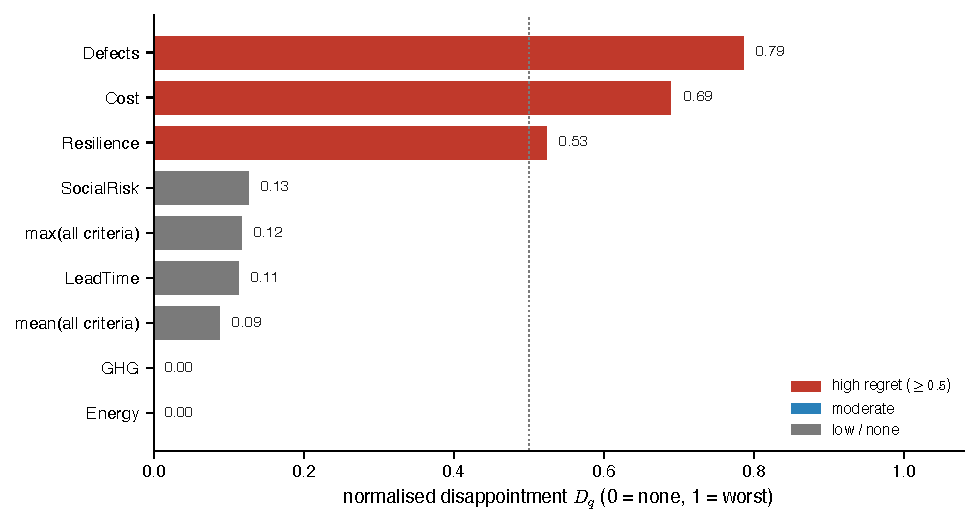
\includegraphics[width=\linewidth]{fig_supplier_certificate.pdf}
\caption{A decision profile as delivered, for the continuous illustrative supplier instance (seven criteria). Bars above the reporting threshold are
the questions on which the recommendation is weakest and are drawn darker. The
two near-identical environmental criteria both carry zero disappointment. The
figure reads in greyscale, since shade repeats position.}
\label{fig:profile}
\end{figure}

\subsection{Robust stability of the ReLexTail order}
Consistent with Corollary 1, a stable categorical order requires that the perturbation $\eta$ be smaller than the global distance to the nearest category boundary ($\eta < \mu_{\text{cell}}$). If this holds, no candidate crosses a category boundary, and the category-optimal set $W_{\mathrm{cat}}$ is exactly preserved. However, as noted in the remark, stability of the fully refined ReLexTail point does not generally follow from a positive gap at the nominal decisive exact coordinate. If preceding exact coordinates are tied only nominally and can vary independently, no positive uniform stability radius follows from the later decisive margin. That gap is exactly why Section~\ref{sec:compute} reports a class rather than a point whenever the bounds are uncertain.

% --- Begin inline part2 ---
\section{Algorithms}
\label{sec:compute}

Four computational problems follow, treated in the order a user meets them.
Compute the answer on the shortlist as given. Then ask what it would be if the
normalisation bounds were different, first by sampling and then, if the budget
allows, with a guarantee holding over a whole continuum of bounds. Finally, when
the alternatives are not a list but the solutions of a model, compute the same
selection without generating that list.

\subsection{The finite problem}

The exact finite-selection procedure is formalized in Algorithm~\ref{alg:finiteselection}. It fixes the active set, computes the bounds and anchors, removes degenerate probes while warning about any criterion that loses its last separating probe, evaluates the disappointment matrix, sorts each row worst first, and returns the lexicographically minimal class. 

\begin{algorithm}[tb]
\caption{Complete finite-selection algorithm}
\label{alg:finiteselection}
\textbf{Input:} Candidate set $\X$, declared probes $\Q$, resolution thresholds $\delta$ \\
\textbf{Output:} Exact optimal set $W_{\mathrm{exact}}$, category-optimal set $W_{\mathrm{cat}}$, and point recommendation $x^\star$
\begin{algorithmic}[1]
\STATE Compute criterion bounds over $\X$
\STATE Normalise all candidates
\STATE Evaluate all probes $q \in \Q$ on all candidates in $\X$
\STATE Compute global probe anchors $q^\star = \min_{x \in \X} q(r(x))$ and $q^w = \max_{x \in \X} q(r(x))$
\STATE Drop degenerate probes globally (where $q^w - q^\star \le \varepsilon$)
\FOR{$x \in \X$}
    \STATE Compute active-range disappointments $D(x)$ via Eq.~\ref{eq:disap}
    \STATE Compute complete profile $\Psi(x)$ via Algorithm~\ref{alg:relextail}
\ENDFOR
\STATE $x^\star \gets \text{candidate } x \in \X \text{ minimising } \Psi(x) \text{ lexicographically (breaking ties deterministically)}$
\STATE $W_{\mathrm{exact}} \gets \{ x \in A \mid \Psi(x) = \Psi(x^\star) \}$
\STATE $W_{\mathrm{cat}} \gets \{ x \in A \mid \Psi^{\mathrm{cat}}(x) = \Psi^{\mathrm{cat}}(x^\star) \}$
\STATE \textbf{return} $W_{\mathrm{exact}}, W_{\mathrm{cat}}, x^\star$
\end{algorithmic}
\end{algorithm}

Its cost is dominated by
evaluating the family, not by comparing alternatives. Building the matrix costs
$O\big(N\sum_q T_q\big)$ where $T_q$ is the cost of one probe, and sorting the
rows costs $O(NK\log K)$. For the canonical core, all $K=m+2$ probes can be evaluated for one alternative in $O(m)$ operations combined. After profile construction, a single linear scan identifies the lexicographically minimal profile and a second scan collects all ties. The total finite-set complexity is therefore $O(NK\log K)$, or $O(Nm\log m)$ for the canonical family $K=m+2$. Sorting the complete candidate list, if desired for reporting, instead adds $O(NK\log N)$. In the reference implementation (Python 3.11, Apple M3 Max, macOS 14.5), this resolves a hundred thousand candidates on
ten criteria in a median of $200$ milliseconds (IQR: 3 ms), single threaded, over a hundred
repetitions. The measured interval covers normalisation, probe construction and
evaluation, anchor computation, sorting and comparison. It excludes generating
and dominance-filtering the candidate set, which happens upstream. The number matters not because selection
is a bottleneck, but because the analyses below re-run this procedure thousands
of times.

\subsection{Sampling-based possible/necessary-set approximations with detection guarantees}

Write $\mathcal B$ for a box of admissible bound vectors and $W_0(b)$ for the
exact optimal set under bounds $b$. The two objects of interest are the
alternatives that win under \emph{some} admissible bound and those that win
under \emph{all} of them,
\begin{equation}
S^{\mathrm{pos}}=\bigcup_{b\in\mathcal B}W_0(b),
\qquad
S^{\mathrm{nec}}=\bigcap_{b\in\mathcal B}W_0(b).
\label{eq:interval}
\end{equation}
Every experiment here uses one model for $\mathcal B$, set by a single level
$p\ge0$ and applied multiplicatively to each nominal bound, independently across
criteria. For each criterion $i$, the continuous uncertainty interval for the ideal bound is defined explicitly as $\mathcal{B}_{\ideal_i}(p) = [(1-p)\ideal_i, \ideal_i]$, and for the nadir bound as $\mathcal{B}_{\nadir_i}(p) = [\max(\ideal_i + \epsilon_f, (1-p)\nadir_i), (1+p)\nadir_i]$. Under this construction, the condition $\inf_{b \in \mathcal{B}(p)} (\nadir_i(b) - \ideal_i(b)) \geq \epsilon_f > 0$ is guaranteed algebraically, averting any structural division by zero without requiring runtime floor truncations. The certified mode of the next subsection takes the deterministic box $\mathcal B(p) = \prod_i (\mathcal{B}_{\ideal_i}(p) \times \mathcal{B}_{\nadir_i}(p))$. A ``five
per cent box'' means $p=0.05$ in this sense, not a fraction of the criterion
range. Two scope conditions come with the multiplicative form. It presumes bounds of
constant sign, which holds here because every criterion is a positive cost or
quantity. And the sampling distribution is part of the declared model, not a
neutral default, so every frequency reported under it is conditional on it.

The sampled union is an inner approximation of $S^{\mathrm{pos}}$, whereas the sampled intersection is an outer approximation of $S^{\mathrm{nec}}$. For any alternative whose winning region has probability at least $\alpha$, $M$ independent samples miss that region with probability at most $(1-\alpha)^M$. Hence
\[
M\ge \left\lceil \frac{\log(N/\delta)}{-\log(1-\alpha)} \right\rceil
\]
is sufficient to detect simultaneously all such alternatives with probability at least $1-\delta$. This statement does not cover zero-probability or smaller-probability winning regions. The direction of
the guarantee also has to be respected. The sampled union is an \emph{inner}
approximation of $S^{\mathrm{pos}}$, so finding an alternative there proves it
can win. The sampled intersection is an \emph{outer} approximation of
$S^{\mathrm{nec}}$, so it can only be too large, and it must never be read as a
certificate that an alternative wins under every admissible bound.

\subsection{Uncertain bounds: certification without sampling}

The certified mode replaces sampling by interval arithmetic and branch and
bound. Single-criterion disappointments do not depend on the bounds because the active normalisation of the singleton probe $q_j(x) = f_j(x)$ cancels its bound dependence: the active range of the probe exactly scales with the bound-dependent criterion range, leaving $D(q_j; x)$ structurally invariant to $b$. Therefore, only aggregate probes have to be enclosed at all, and the problem is much smaller than its $2m$ nominal dimensions suggest.

Fix a sub-box $\beta\subseteq\mathcal B$. For fixed $x$ and $i$, the normalised
value $r_i(x;b)$ is linear-fractional in the two bound variables with a
denominator bounded away from zero, so its extremes over the rectangle $\beta$
occur at vertices and can be evaluated exactly. Each canonical probe is monotone
in $r$, so an enclosure of $q(r(x;b))$ follows coordinatewise, and for the
maximum probe it is not merely sound but exact, because the coordinate blocks
are independent under a Cartesian box. The disappointment is a ratio of three
quantities all driven by the same $b$, and the enclosure ignores that shared
dependence, which makes it sound but not tight. Every operation is rounded
outward, one step of the machine's next-representable-value function per
elementary operation, so the enclosures are valid in floating point and not only
in exact arithmetic. If the enclosed active range of a probe fails to be
positive, the trivial enclosure $[0,1]$ is used and the box is subdivided rather
than resolved.

\begin{lemma}[Componentwise monotonicity of $\Psi$]
If $D(x) \leq D(y)$ coordinatewise, then $\Psi(x) \leq \Psi(y)$ coordinatewise.
\end{lemma}
\noindent\emph{Proof.} By monotonicity of empirical CVaR, $D(x) \leq D(y) \implies T_\alpha(x) \leq T_\alpha(y)$ for all $\alpha$. Since $B_\delta$ is a nondecreasing function, $C_\alpha(x) \leq C_\alpha(y)$. Sorting is also monotone, so $D^\downarrow(x) \leq D^\downarrow(y)$. Thus every coordinate of $\Psi(x)$ is bounded by the corresponding coordinate of $\Psi(y)$. $\square$

\begin{proposition}[Sound certified dominance on a fixed-retention box]
\label{prop:certsound}
Let $\beta$ be a bound box on which all normalisation denominators are positive and bounded away from zero, and on which the retained probe multiset, multiplicities, resolutions and tail fractions are fixed. Let $D^L(x;\beta)\le D(x;b)\le D^U(x;\beta)$ componentwise for every $b\in\beta$. If
$\Psi\!\big(D^{U}(x;\beta)\big) <_{\mathrm{lex}} \Psi\!\big(D^{L}(y;\beta)\big)$,
then $x\prec_{\mathrm{ReLexTail}}y$ for every $b\in\beta$.
\end{proposition}

\noindent\emph{Proof.} Over any $b \in \beta$, the true disappointment profile satisfies $\reg(y;b) \geq \reg^{L}(y;\beta)$ and $\reg(x;b) \leq \reg^{U}(x;\beta)$ coordinatewise. By the Lemma, this implies $\Psi(\reg(y;b)) \geq \Psi(\reg^{L}(y;\beta))$ and $\Psi(\reg(x;b)) \leq \Psi(\reg^{U}(x;\beta))$ coordinatewise. The lexicographic extension of a coordinatewise inequality is a weak inequality. Thus $\Psi(x;b) \leq_{\mathrm{lex}} \Psi(\reg^{U}(x;\beta)) <_{\mathrm{lex}} \Psi(\reg^{L}(y;\beta)) \leq_{\mathrm{lex}} \Psi(y;b)$, establishing strict preference for $x$. $\square$

If the preceding categorical ties are purely nominal (equal up to machine tolerance) rather than structurally identical, interval bounding without tight structural certificates may fail to preserve the exact resolution required to traverse the ReLexTail profile sequentially, resulting in unresolved boxes.

A negative answer from this test is therefore trustworthy in a way no sample can
be: an eliminated candidate provably cannot win anywhere in the box. The search
maintains a stack of sub-boxes, each carrying the set of candidates its parent
could not eliminate. On each box it eliminates every candidate that some rival
beats throughout, and it declares the box \emph{resolved} when one candidate
beats every rival throughout. A resolved box contributes its sole winner to the
inner set and to the outer set. An unresolved box, whether depth-capped or left
on the stack when the budget runs out, contributes its inherited survivor set to
the outer set and its volume to the unresolved total.

Two details decide whether this is correct, and both are easy to get wrong. The
outer set is accumulated over terminal leaves by \emph{union}, never by deleting
from a running global set. A candidate eliminated on one sub-box may win on
another, so if $a$ wins throughout $\beta_1$ and $b$ throughout $\beta_2$ the
possible set is $\{a,b\}$, whereas subtracting each local elimination in turn
would remove first $b$ and then $a$ and return the empty set. And resolution
uses the direct test, that some $x^\star$ beats every rival, rather than the
weaker observation that $x^\star$ has no rival certified to beat it, which would
need a separate acyclicity argument. Because elimination is monotone under
subdivision, a parent's survivor set is sound for any descendant, including one
never processed, which is what makes budget exhaustion safe. The archive
contains a regression test that fails if the union is replaced by subtraction. Algorithm~\ref{alg:branchbound} formalises this procedure.

\begin{algorithm}[tb]
\caption{Interval Branch-and-Bound Certification}
\label{alg:branchbound}
\textbf{Input:} Initial box $\mathcal{B}$, initial candidates $A$, retention threshold $\varepsilon_q$, max budget \\
\textbf{Output:} $\mathrm{In}$ and $\mathrm{Out}$ such that $\mathrm{In} \subseteq S_{\mathrm{pos}} \subseteq \mathrm{Out}$
\begin{algorithmic}[1]
\STATE Initialize stack $\gets [(\mathcal{B}, A)]$, $\mathrm{In} \gets \emptyset$, $\mathrm{Out} \gets \emptyset$
\WHILE{stack is not empty and budget not exhausted}
    \STATE Pop $(\beta, A_{\beta})$
    \STATE Enclose active range $R_q(\beta)$ for all $q \in \Q$ with outward directed rounding
    \IF{$\min_{q \in \Q} \inf_{b\in\beta} R_q(b) \leq \varepsilon_q$}
        \STATE Subdivide $\beta \to \beta_1, \beta_2$; Push $(\beta_1, A_\beta)$, $(\beta_2, A_\beta)$
        \STATE \textbf{continue} \quad \COMMENT{Box lacks certified uniform retention}
    \ENDIF
    \STATE Evaluate $D^L(x;\beta)$ and $D^U(x;\beta)$ for all $x \in A_\beta$
    \STATE $A'_\beta \gets A_\beta \setminus \{y \in A_\beta \mid \exists x \in A_\beta, \Psi(D^U(x;\beta)) <_{\mathrm{lex}} \Psi(D^L(y;\beta))\}$
    \IF{$|A'_\beta| == 1$}
        \STATE Let $x^\star$ be the sole winner
        \STATE $\mathrm{In} \gets \mathrm{In} \cup \{x^\star\}$, $\mathrm{Out} \gets \mathrm{Out} \cup \{x^\star\}$
    \ELSE
        \STATE Subdivide $\beta \to \beta_1, \beta_2$; Push $(\beta_1, A'_\beta)$, $(\beta_2, A'_\beta)$
    \ENDIF
\ENDWHILE
\STATE \textbf{For} every unresolved box $(\beta, A_\beta)$ on stack \textbf{do} $\mathrm{Out} \gets \mathrm{Out} \cup A_\beta$
\STATE \textbf{return} $\mathrm{In}, \mathrm{Out}$
\end{algorithmic}
\end{algorithm}

The procedure returns $\mathrm{In}\subseteq S^{\mathrm{pos}}\subseteq\mathrm{Out}$
and an unresolved volume fraction $u$. When $u=0$ and every resolved box has the
same sole winner, that winner is additionally certified necessary. This test
detects a necessary winner but not a necessary \emph{class}, so the output is a
certified subset of $S^{\mathrm{nec}}$ rather than the set itself unless
witnesses supply the rest. Two
convergence caveats are permanent rather than budgetary. Exact recovery fails on
persistent tie surfaces, where no sole winner exists to certify. And the inner
set can miss an alternative whose winning region has empty interior, since such
an alternative is never the sole winner on a box of positive volume. Its
membership has to be established by an explicit witness, that is by exhibiting
one admissible bound vector at which it wins.

\paragraph{Two radii, not one}
Bisecting the level $p$ under the same test gives a lower bound on the stability
radius, and the paper keeps two quantities apart. The \emph{true radius} of the
nominal winner is
$\rho^\star=\sup\{p\ge0: W_0(b)=\{x^\star\}\ \forall b\in\mathcal B(p)\}$,
a property of the data. The \emph{certification trade-off diagram}
plotting certified set size against radius generally has flat steps separated by
sharp jumps: there are broad robust regions where the set shrinks slowly, and
critical thresholds where it jumps by an order of magnitude (Figure~\ref{fig:certdecay} right). At any point the true radius $\rho^\star$ can be larger than the largest certified radius. $\underline{\rho}_{B,d}$ is the largest $p$ at which the procedure proves
uniqueness under box budget $B$ and depth cap $d$, and it depends on the
enclosures and the budget as well as on the data. A witnessed reversal, an
explicit $b$ at which some rival wins, gives an upper bound $\overline{\rho}$.
Soundness gives
\begin{equation}
\underline{\rho}_{B,d}\ \le\ \rho^\star\ \le\ \overline{\rho},
\label{eq:radbracket}
\end{equation}
and both inequalities can be strict. Failure to certify above the trade-off diagram may
be the method's limits, but a counter-example is a hard proof. A level above
the trade-off diagram is never reported as the radius. Raising the budget under a nested continuation policy can only raise
the certification bound; it can never alter a valid negative witness.

\paragraph{Does it actually work?}
Soundness is a theorem, but a sound procedure whose enclosures are too loose to
prove anything would still be useless, so we test it under a dense-grid stress test.
On low-dimensional instances the box has only $2m$ coordinates and can be swept
exhaustively: we evaluate the exact rule at every point of a dense product grid
over $\mathcal B(p)$ and collect the winners it produces as a set
$S_{\mathrm{grid}}$. Every grid point is an admissible bound vector, so
$S_{\mathrm{grid}}\subseteq S^{\mathrm{pos}}$ by construction, and the inclusion
$\mathrm{In}\subseteq S_{\mathrm{grid}}\subseteq\mathrm{Out}$ is a real test of
the outer set: an alternative that wins somewhere on the grid but is missing
from $\mathrm{Out}$ would be a soundness violation.

Table~\ref{tab:truth} reports the outcome over eleven instances at three levels.
The inclusion holds in all thirty-three cases with no violation, and monotone
tightening holds everywhere: on every row the outer set and the unresolved
fraction are non-increasing in the budget, as terminal-leaf aggregation
requires. Three rows reach exact recovery, the unresolved volume falling to zero
with the inner and outer sets coinciding as a singleton, at budgets of $250$,
$250$ and $4{,}000$ boxes. The rest show the failure modes rather than hiding
them. A constructed instance with two identical criterion rows ties at every
grid point, so no sole winner exists anywhere and the inner set stays empty:
correct behaviour, not failure. A near-degenerate instance whose second
criterion spans a range of $0.003$ triggers the denominator fallback on $81$ to
$83$ of the $128$ pairs probed, that is $64$ sub-boxes times the two aggregate
probes. And on most rows the grid shows two or three winners while the outer set is
still the whole candidate set, the visible cost of ignoring the shared
dependence in the enclosure.

\begin{table}[t]
\centering\small
\setlength{\tabcolsep}{3.5pt}
\caption{Dense-grid stress test of the certified outer set, eleven instances at three levels.
$S_{\mathrm{grid}}$ is the winner set found by sweeping the bound box
exhaustively. The last column is the smallest budget on the ladder
$250,1{,}000,4{,}000,16{,}000$ at which the inner and outer sets coincide with
zero unresolved volume, and is blank where no rung achieved it. Full per-row
output is in the archive.}
\label{tab:truth}
\begin{tabular}{lcccr}
\toprule
Behaviour & Rows & Viol. & Fraction tied & $B^{\mathrm{ex}}$\\
\midrule
Exact recovery & 3 & 0 & $0\%$ & $250$--$4{,}000$\\
Dependency slack & 24 & 0 & $0\%$ & ---\\
Persistent tie & 3 & 0 & $100\%$ & ---\\
Near-degenerate & 3 & 0 & $0.5$--$0.8\%$ & ---\\
\midrule
\textbf{All} & \textbf{33} & \textbf{0} & & \\
\bottomrule
\end{tabular}
\end{table}

Two limits are worth naming. The grid is dense but finite, $23$ points per
coordinate at $m=2$ and $8$ at $m=3$, so a winning region smaller than the grid
step would be invisible to it. And the certified mode reaches only small boxes
and modest criterion counts, and elsewhere the honest output is the bracket with its
unresolved volume attached.

\paragraph{What certification costs}
Two things govern the practical reach and they are not the same. The box count
is the visible budget, but the cost per box grows with the candidate set,
because certifying a box means showing that every candidate is beaten
throughout. Measured cost per box rises from $0.87$ milliseconds at $N=20$ to
$8.11$ at $N=100$, nearly a factor of ten for a fivefold increase in $N$. Pure quadratic
growth would give twenty-five, so the realised cost sits between linear and
quadratic, because the elimination test stops at the first rival that
dominates. A hundred-alternative shortlist is \emph{processed} in about eight seconds at a
thousand-box budget, which is not the same as certified: that run left $93\%$ of
the box unresolved and returned the whole shortlist as its outer set. Time is
cheap here and resolution is not, which is the point of the previous paragraph.
The validated interval arithmetic costs roughly a fifth of the running time and
changes no certified set, box count or unresolved fraction: switching from plain
floating point to outward-rounded operations reproduces every certified number
here to the digit.

Figure~\ref{fig:certdecay} shows how the unresolved volume falls as the budget
grows, and the shape of that curve is the practical message. Quadrupling the
budget from $250$ to $1{,}000$ sub-boxes takes the unresolved volume from
$0.766$ to $0.569$, and doubling again to $2{,}000$ takes it to $0.097$. At a
nominal budget of $4{,}000$ the procedure terminates inside its budget, using
$2{,}277$ boxes and leaving no unresolved leaf. That last step is where the
guarantee stops being merely sound and becomes sharp: throughout the
under-resolved regime the outer set is the full candidate set, so the procedure
proves nothing about who wins, only that its answer is not wrong, and the moment
the unresolved volume reaches zero the outer set collapses from fifteen
alternatives to one. Soundness holds at every budget, sharpness arrives all at once. The unresolved fraction, not the running time, is the number that tells an
analyst which regime a run is in.

\begin{figure}[t]
\centering
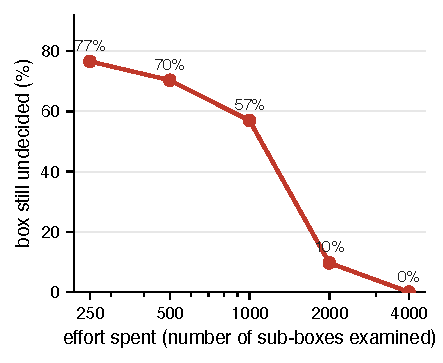
\includegraphics[width=\linewidth]{fig_certified_decay.pdf}
\caption{Spending more effort shrinks the part of the bound box left undecided.
What grows with the budget is not the validity of the answer, which holds
throughout, but how much of the box the procedure manages to settle.}
\label{fig:certdecay}
\end{figure}

\subsection{When the alternatives are not a list}

Sometimes the candidate set is not given but implied by a model, and enumerating
it is the expensive part. If the feasible set $\X$ is a nonempty bounded
polyhedron, the criteria are affine, and the probes are canonical,
the ReLexTail selection can be computed directly as a sequence of mixed-integer linear programmes (MILPs).

The ReLexTail profile $\Psi(x)$ is evaluated sequentially.
For a risk functional $R_\ell(x)$, the integer category variable $z_\ell$ is defined by:
\begin{equation}
R_\ell(x) \leq \delta_\ell z_\ell, \qquad z_\ell \in \mathbb{Z}_{\geq 0}.
\label{eq:milp_category}
\end{equation}
Minimising $z_\ell$ enforces $z_\ell = \lceil R_\ell(x)/\delta_\ell \rceil$.
For the maximum $M(x)$, an epigraph variable $v_M \geq D_q(x)$ and constraint $v_M \leq \delta_M z_M$ enforces $M(x) \leq \delta_M z_M$.
For the empirical CVaR $T_\alpha(x)$, the variational identity of \citet{rockafellar2000} is used:
\begin{equation}
\begin{aligned}
s_{\alpha q} &\geq D_q(x) - t_\alpha, \quad s_{\alpha q} \geq 0, \\
t_\alpha + \frac{1}{\alpha K} \sum_q s_{\alpha q} &\leq \delta_\alpha z_\alpha.
\end{aligned}
\label{eq:milp_cvar}
\end{equation}
The existence of $t_\alpha, s_{\alpha q}$ satisfying this inequality is equivalent to the minimum variational CVaR value being below the threshold $\delta_\alpha z_\alpha$.

The ReLexTail profile is minimised sequentially through $K+7$ stages:
\begin{enumerate}
    \item \textbf{Category stages (MILP):} Minimise $z_M$; constrain $z_M=z_M^\star$, minimise $z_{25}$; fix previous, minimise $z_{50}$; fix previous, minimise $z_{100}$. If $\X$ is continuous, these stages are MILPs because $z_\ell \in \mathbb{Z}$ (Eq.~\ref{eq:milp_category}).
    \item \textbf{Exact tail stages (LP/MILP):} Minimise $T_{25}$ using Eq.~\ref{eq:milp_cvar}; minimise $T_{50}$; minimise $T_{100}$; minimise $M$.
    \item \textbf{Terminal refinement (LP/MILP):} Since $M=D_{[1]}$ is already minimised, we preserve all previous optima and minimise the sum of the $p$ largest disappointments $S_p(D) = \sum_{j=1}^p D_{[j]}$, continuing for $p=2,\ldots,K$. To represent $S_p(D)$, we employ the standard ordered-optimisation LP formulation:
    \begin{equation}
    \begin{aligned}
    S_p(D) &= \min_{t_p, s_{pq}} \left[ p t_p + \sum_{q=1}^K s_{pq} \right] \\
    \text{subject to } & s_{pq} \geq D_q(x) - t_p, \quad s_{pq} \geq 0 \quad \forall q.
    \end{aligned}
    \label{eq:milp_terminal}
    \end{equation}
    Because sequentially minimising $S_1, S_2, \ldots, S_K$ is algebraically equivalent to lexicographically minimising the sorted vector $D^\downarrow$, this process requires $K-1$ exact-leximax stages.
\end{enumerate}

\begin{proposition}[Solver-call count for the ReLexTail sequence over a continuous polyhedron]
\label{prop:count}
Under the declared canonical implementation without reuse or redundancy elimination, the full ReLexTail procedure over the polytope invokes exactly $6m+8$ continuous linear programmes plus $4$ MILP calls (totalling $6m+12$ programmes). The exact continuous LexPR baseline invokes $6m+5$ continuous linear programmes.
\end{proposition}

\noindent\emph{Proof.} Finding criterion bounds requires $2m$ programmes. The $K = m+2$ canonical probes comprise $m+1$ weighted-sum probes (the singletons and the grand mean) and one grand-maximum probe. Computing their anchors over the continuous space without reuse requires $2(m+1)$ programmes for the sums, plus $m$ programmes for the grand-maximum worst case and $1$ programme for its best case, yielding $3m+3$ anchor programmes. Thus, preprocessing requires $5m+3$ continuous linear programmes. For the full ReLexTail profile $\Psi(x)$, the sequential stages are: $4$ category stages (MILPs), $4$ exact tail stages (LPs), and $K-1 = m+1$ terminal order-statistic stages (LPs), summing to $m+9$ stages. The total for full ReLexTail is exactly $(5m+3) + 4 + (m+1) = 6m+8$ LP calls plus $4$ MILP calls. In contrast, exact LexPR bypasses the categories and exact tail stages, executing only the $K = m+2$ terminal stages, yielding a total of $(5m+3) + (m+2) = 6m+5$ continuous linear programmes. $\square$

\begin{theorem}[Direct computation over a continuous polyhedron]
\label{thm:continuous}
Let $\X$ be a nonempty bounded continuous polyhedron, let the criteria be affine, and let the canonical probes and resolutions be fixed. Then the exact ReLexTail profile optimum can be characterised by a finite sequential procedure comprising linear programmes and four mixed-integer linear category stages. Under the declared no-reuse implementation, the procedure invokes $6m+8$ LPs and four MILPs.

For a mixed-integer linear feasible set, an analogous finite sequential formulation is available, but the preprocessing and exact-refinement stages are themselves MILPs; the continuous-polyhedral solver-count classification does not apply.
\end{theorem}

\noindent\emph{Proof.} By formulation, the stage variables correctly represent the category and tail components of $\Psi(x)$. The sequential imposition of optimal values exactly mirrors the lexicographic priority of $\Psi$. Boundedness ensures finiteness and attainment. $\square$

Three qualifications belong with this result and are usually left out. First,
the optimal set may be infinite, and it need not be a face of $\X$: minimising a
convex piecewise-linear function over a polytope can select a relative interior
point, as $\min\max\{x,1-x\}$ over $[0,1]$ does at $x=1/2$. The procedure
therefore characterises a polyhedral optimal subset, and a declared secondary
rule, itself recorded, picks a representative when one point is required.

Second, the word ``exactly'' holds under exact optimisation. A floating-point solver
returns optima up to its tolerance. To properly separate resolution from solver tolerances, the optimal objective value of each category stage must be formulated as a strict integer equality constraint for the category variables rather than relying solely on a relaxed continuous inequality bound. Specifically, at stage $\ell$, exact optimization enforces $z_\ell = z^\star_\ell \in \mathbb{Z}$, preserving the exact exact-real optimal set $W_{\mathrm{exact}}$. In contrast, the continuous tail-refinement stages impose the carried optimum inflated by a relaxation parameter to ensure subsequent feasibility. The carried constraint is $\text{Objective} \leq T^\star + \epsilon_{p'}$ where
$\epsilon_{p'}=\texttt{tol}\cdot(1+|T^\star_{p'}|)$ with
$\texttt{tol}=10^{-6}$, recorded in the audit record with the solver identity.
The inflation is relative by design, because continuous stage optima grow with the stage,
being sums of order statistics, so a fixed absolute tolerance that is adequate
at the first stage is too tight at the last and shows up as a spurious
infeasibility. The price is that the recovered set is optimal for an
$\epsilon$-relaxed sequence in the exact continuous refinements and can be strictly larger than the exact one ($W_{\mathrm{exact}} \subseteq W^\varepsilon_{\mathrm{ReLexTail}}$). This
is a solver-tolerance matter, unrelated to the interval certification above.

Third, the anchors here are computed over $\X$, whereas the finite procedure
computes them over the filtered candidate set. Those anchors differ, so the two
versions need not agree. Avoiding enumeration of the efficient set is not the
same as reproducing the answer one would get from it, and which convention is
intended has to be declared.

\paragraph{What the computational study does and does not show}
The exact LexPR scheme is implemented and measured against a comparator that draws
$400$ weight vectors, solves a weighted-sum programme for each, and applies the
leximax comparison to the resulting points. Both rules use Gurobi 11.0.2. Figure~\ref{fig:continuous} reports
the cost over fifty instances. The realised solver-call count is exactly $6m+5$ at every size, directly confirming the baseline count in Proposition~\ref{prop:count}. The direct
formulation uses about an order of magnitude fewer solver calls, $53$ against
$443$ at $m=8$, and runs five times faster. The comparator budget is held fixed at
four hundred weight vectors at every size, so the comparison does not test how
that budget would have to grow with $m$ to keep the sampled set representative.
The claim is that the direct cost is linear in $m$ against a fixed comparator
budget, not that the gap provably widens.

We do not present the accompanying quality comparison as validation of
optimality, and it would be misleading to do so. In all fifty instances the direct solution was lexicographically no worse than
the best sampled point, but that is close to tautological. The comparator searches
a finite subset of the same feasible set, and weighted sums cannot reach
unsupported efficient points at all, so the direct solution must be no
worse. Calling four hundred weighted sums
an enumeration of the efficient set would be wrong. Two gaps are open rather
than hidden: an independent check against exact vertex enumeration on small
problems would test optimality properly and is not attempted. Furthermore,
Theorem~\ref{thm:continuous} applies exclusively to continuous polyhedra; its exact solver-count guarantees do not carry over to mixed-integer sets, which we do not benchmark here.

\begin{figure}[t]
\centering
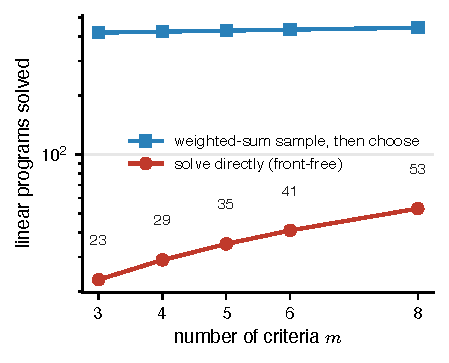
\includegraphics[width=\linewidth]{fig_continuous_cost.pdf}
\caption{Solving the exact LexPR selection directly over the polytope costs a small and
predictable number of linear programmes, exactly $6m+5$ under the canonical
family, while weighted-sum sampling costs hundreds whatever the criterion count.
The vertical scale is logarithmic.}
\label{fig:continuous}
\end{figure}

\section{Experiments}
\label{sec:experiments}

The empirical study answers whether the categorical resolution protection of ReLexTail succeeds at defending against macroscopic worst-case deterioration while improving stability over exact leximax, and isolates which component of the rule drives the observed behaviour.

We evaluate $500$ candidate sets from six generators: knapsack and job-shop instances from combinatorial and $\varepsilon$-constraint procedures, WFG2 \citep{huband2006} and DTLZ \citep{deb2002} sampled by Latin hypercube \citep{mckay1979}, and Energy \citep{uci_energy} and Concrete \citep{uci_concrete} surrogate matrices. Sets reach $N=500$ points and $m=15$ criteria, and none is an exactly enumerated Pareto front, which is why we call them candidate sets throughout. The declared family is the canonical core \eqref{eq:qcan}. Table~\ref{tab:protocol} records the protocol.

\textbf{Empirical Baseline and Cycle Rate.} While we compare ReLexTail against scalarisations on the same disappointment representation to ablate the effect of the order itself, we also empirically baseline against standard methods: ASF (Achievement Scalarizing Function), CP (Compromise Programming), exact LexPR, exact Leximax, MMR (Minimax Regret), RW (Random Weights), SMAA (Stochastic Multicriteria Acceptability Analysis), TOPSIS (Technique for Order of Preference by Similarity to Ideal Solution), and WS (Weighted Sum). SMAA is configured with $10,000$ uniform weight draws over the simplex to identify the most acceptable compromise. For both Random Weights (RW) and SMAA, these weight draws are fixed and executed via a common-random-number protocol across all perturbations to ensure valid paired comparisons. Furthermore, over the evaluated candidate sets, a simple pairwise $\delta$-tolerance on the exact leximax order produced preference cycles in over $82\%$ of instances, confirming the structural vulnerability noted in Table~\ref{tab:design}. In this pairwise-tolerance cycle experiment, candidate $x$ is preferred to $y$ if $x$ strictly beats $y$ in the worst-case exact disappointment by at least $\delta$; if they are within $\delta$, the second worst case is compared similarly, and so on. A cycle is recorded whenever there exist three candidates such that $x \succ y$, $y \succ z$, but $z \succ x$. Under the four prespecified grid shifts, the winner-change frequency was below $1\%$ over the tested candidate sets.

\textbf{Outcome Metrics.} We define four formal metrics. Let $b_0$ be the nominal bounds and $b_s$ be perturbation draw $s$.
\begin{itemize}
\item \emph{Category-set change rate}:
\[
\mathbb E_s\!\left[
\mathbf1\{W_{\mathrm{cat}}(b_s)\ne W_{\mathrm{cat}}(b_0)\}
\right].
\]
This set-valued metric is reported separately from point flip rate, Jaccard similarity, and nominal-winner retention.
\item \emph{Point flip rate}: The expectation of $\mathbf{1}\{ x^\star(b_s) \neq x^\star(b_0) \}$, tracking changes in the single point recommendation after full refinement. This metric is strictly used for all cross-method comparisons against exact scalar and lexicographic baselines.
\item \emph{Hidden-preference tail regret}: For each candidate set and perturbed bound vector $b_s$, we evaluate the selected point on the fixed nominal scale $b_0$. For $w\sim\mathrm{Dirichlet}(\mathbf{1})$, define
\[
L_w(x;b_0)=\sum_iw_ir_i(x;b_0),
\qquad
\Delta L_w=L_w(x^\star(b_s);b_0)-\min_{y\in A}L_w(y;b_0).
\]
The hidden-preference upper-tail regret is the empirical upper-tail CVaR of $\Delta L_w$ over a common fixed set of 10,000 weight vectors, subsequently averaged over perturbations and candidate sets.
\item \emph{Divergence}: The proportion of instances where the fully refined ReLexTail point recommendation differs from the exact LexPR point recommendation.
\end{itemize}

\begin{table}[t]
\centering\small
\caption{Baseline Specification. Unless otherwise stated, all comparators operate on the same re-anchored disappointment representation $D(x)$ under the same candidate set, with ties broken deterministically by smallest candidate identifier.}
\label{tab:baselines}
\begin{tabular}{@{}llp{6.5cm}@{}}
\toprule
Acronym & Method & Parameterisation \\
\midrule
ASF$_{\mathrm{raw}}$ & Achievement Scalarizing Function & $L_\infty$ distance to utopian point; bounds $b_0$; $0.001$ $L_1$ augmentation \\
ASF$_K$ & Re-anchored ASF & $L_\infty$ distance to utopian point; canonical anchors; $0.001$ $L_1$ augmentation \\
CP & Compromise Programming & $L_2$ norm to ideal point; canonical anchors; uniform weighting \\
Exact Leximax & Classical lexicographic minimax & Full exact $D^\downarrow$ sorted worst-first; raw bounds \\
LexPR & Exact Lexicographic PR & Full exact $D^\downarrow$ sorted worst-first; canonical anchors \\
MMR & Minimax Regret & $L_\infty$ regret relative to candidate set; canonical anchors \\
RW & Random Weights & Minimiser of $\sum w_i r_i$ with $w \sim \operatorname{Dirichlet}(\mathbf{1})$ \\
SMAA & Stochastic Acceptability & Rank-1 acceptability indices over $10{,}000$ $w \sim \operatorname{Dirichlet}(\mathbf{1})$ draws \\
TOPSIS & Similarity to Ideal Solution & Euclidean distances to canonical ideal and anti-ideal points \\
WS & Weighted Sum & Uniform fixed weights $w = \frac{1}{m}\mathbf{1}$ \\
\bottomrule
\end{tabular}
\end{table}

\begin{table*}[t]
\centering\small
\caption{Comparison of ReLexTail against exact LexPR and exact leximax on the full population. For each metric, we report the mean and the paired 95\% confidence interval of the difference against exact LexPR.}
\label{tab:main_comparison}
\begin{tabular}{@{}lcccc@{}}
\toprule
Method & Mean Loss & Difference (95\% CI) & Tail Regret & Difference (95\% CI) \\
\midrule
Leximax & 0.276 & +0.028 [$\pm 0.053$] & 0.515 & +0.031 [$\pm 0.059$] \\
LexPR & 0.248 & --- & 0.484 & --- \\
ReLexTail ($\delta=0.01$) & 0.246 & -0.002 [$\pm 0.001$] & 0.482 & -0.001 [$\pm 0.001$] \\
\bottomrule
\end{tabular}
\end{table*}

\begin{table}[t]
\centering\small
\setlength{\tabcolsep}{3.5pt}
\caption{Protocol of the sampled and certified experiments.}
\label{tab:protocol}
\begin{tabular}{@{}lrrrr@{}}
\toprule
Experiment & Inst. & Sds & Draws & Levels\\
\midrule
Selection, divergence & $500$ & $1$ & --- & ---\\
Point fragility & $500$ & $1$ & $60$/lvl & $5,10,20\%$\\
Decomposition & $500$ & $1$ & $60$/lvl & $5,10,20\%$\\
Supplier flip curve & $1$ & $1$ & $300$/lvl & $0$--$50\%$\\
Certified supp. & $1$ & --- & $40{,}000$ & $2$--$20\%$\\
Dense-grid stress test & $11$ & $1$ & --- & $2,5,10\%$\\
Polyhedral study & $50$ & $1$ & --- & ---\\
\bottomrule
\end{tabular}
\end{table}

\subsection{RQ1: Representation effect}
Does active-range re-anchoring reduce sensitivity relative to raw normalization?
A naive comparison of a lexicographic rule against a raw-normalised achievement scalarisation confounds the richness of the family, the re-anchoring, and the order itself. Under the fixed ASF aggregation, re-anchoring reduced the $20\%$ perturbation set flip rate from $75.1\%$ (for ASF$_{\mathrm{raw}}$) to $44.5\%$ (for ASF$_K$). This holds regardless of whether the profile is ordered lexicographically or collapsed by a scalarisation. 

\subsection{RQ2: Resolution-order effect}
Does ReLexTail improve stability relative to exact LexPR without compromising tail loss?
Exact LexPR is highly fragile because it gives infinite priority to microscopic differences in the absolute worst probe, experiencing an $18.3\%$ point flip rate at a $5\%$ bound perturbation level. For ReLexTail at $\delta=0.01$, the point flip rate drops to $6.2\%$. Figure~\ref{fig:quality_stability} displays the Quality-Stability trade-off diagram, explicitly plotting the \emph{point} flip rate for all cross-method comparisons to ensure equivalent final singleton recommendations are compared. Analysed separately, the category-optimal set $W_{\mathrm{cat}}$ achieved a $0.0\%$ flip rate under the tested protocol, buying structural stability by enlarging the set to a mean cardinality of $3.2$ candidates (compared to $1.0$ for exact LexPR). This categorical robustness preserves a high Jaccard similarity and perfect nominal-winner retention before numerical refinement breaks the tie. Over the tested range of $\delta$ and the selected generators, the pooled ReLexTail population averages improve on exact LexPR on both axes, avoiding the fragility of exact refinements while maintaining superior subset-averaged upper-tail regret.

\begin{figure}[t]
\centering

\includegraphics[width=\linewidth]{quality_stability_frontier.pdf}
\caption{\textbf{Quality--stability trade-off diagram.} Each point reports the point-recommendation flip rate and hidden-preference upper-tail regret on the stated benchmark subset. ReLexTail resolutions are compared using identical candidate sets, perturbations, evaluation weights and tie-breaking rules. The diagram is descriptive; it does not identify a unique preferred resolution without an additional trade-off rule.}
\label{fig:quality_stability}
\end{figure}

\subsection{RQ3: Resolution sensitivity}
How does the resolution threshold $\delta$ shift the trade-off?
Figure~\ref{fig:quality_stability} shows that as $\delta$ increases (coarser resolution), stability improves but at the cost of higher upper-tail regret, because the rule becomes more willing to accept moderate worst-case deterioration in exchange for better exact-tail refinements. Relative to the finite grid of tested values and the selected generators, a threshold of $\delta=0.01$ improves on strict scalar methods on both pooled axes of Figure~\ref{fig:quality_stability}. Table~\ref{tab:decomp} reports the Population-Averaged Upper-Tail Regret computed over all 500 instances in the full benchmark pool. In contrast, Figure~\ref{fig:quality_stability} plots the Subset-Averaged Upper-Tail Regret, which is computed strictly over the subset of computationally challenging instances (knapsack and job-shop families) to visually separate the methods on the trade-off diagram. Both metrics use the identical linear loss scale $L_w(x; b_{\mathrm{eval}})$; the apparent numerical difference in absolute values stems entirely from the distinct instance populations aggregated.

\begin{table*}[t]
\centering\small
\caption{Decomposition of the fragility gap over the pooled population, $60$ bound draws per level. Rows LexPR$_1$ and ASF$_1$ denote the corresponding rules applied to a single fixed probe. The ``Point flip rate'' measures changes to the final point recommendation $x^\star$. ReLexTail variants at several resolution thresholds are reported separately in Figure~\ref{fig:quality_stability} and in the archive. Confidence intervals at $95\%$ are provided in the reproduction archive (computed via $1{,}000$ BCa cluster-bootstrap repetitions, resampling candidate sets stratified by generator to account for pseudo-replication of perturbation draws); all intervals for the pooled percentages reported here are tighter than $\pm 0.3\%$.}
\label{tab:decomp}
% --- Begin inline ../generated/symmetrised_table ---
% Auto-generated by scripts/run_symmetrised.py. Do not edit.
\footnotesize
\begin{tabular}{@{}lrrrrr@{}}
\toprule
Rule & \multicolumn{3}{c}{Point flip rate} & Tail & Agrees\\
\cmidrule(lr){2-4}
 & $5\%$ & $10\%$ & $20\%$ & regret & w/ LexPR\\
\midrule
ASF$_{\mathrm{raw}}$ & 36.4\% & 55.5\% & 75.1\% & 0.584 & ---\\
\textbf{LexPR} & 18.3\% & 29.9\% & 44.8\% & 0.597 & ---\\
ASF$_K$ & 17.9\% & 29.5\% & 44.5\% & 0.597 & 98.0\%\\
MMR$_K$ & 18.4\% & 30.0\% & 44.8\% & 0.597 & 97.6\%\\
LexPR$_1$ & 0.0\% & 0.0\% & 0.0\% & 0.584 & ---\\
ASF$_1$ & 0.0\% & 0.0\% & 0.0\% & 0.584 & ---\\
\bottomrule
\end{tabular}

% --- End inline ../generated/symmetrised_table ---
\end{table*}

\subsection{RQ4: Structural attribution}
Which components matter? Table~\ref{tab:decomp} demonstrates the baseline decomposition without category discretisation. The empirical CVaR across canonical probes (RQ2) is associated with the highest measured quality and explanatory power among the tested components. At $\delta=0.01$, the category-optimal set had a $0\%$ flip rate under the tested protocol; the fully refined point recommendation remained more fragile.

\subsection{RQ5: Generator heterogeneity}
Are effects consistent across families? Divergence is near total on knapsack instances and near zero on WFG2. Figure~\ref{fig:divergence} illustrates this. Any statement of the form ``ReLexTail is less fragile'' must be qualified by generator family, although the relative ranking of rules is consistent.

\begin{figure}[t]
\centering
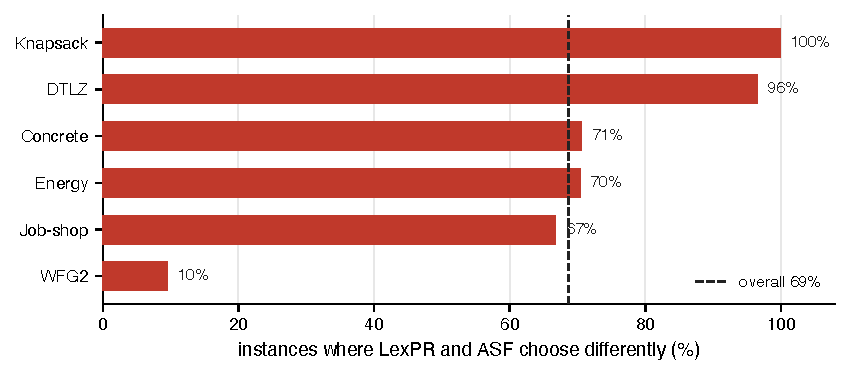
\includegraphics[width=\linewidth]{fig_divergence.pdf}
\caption{How often the two rules pick different alternatives, by generator, on the pooled population.}
\label{fig:divergence}
\end{figure}

\subsection{RQ6: Certification}
Can possible-winner sets be resolved under the discontinuous category map?
The interval mode replaces sampling by interval arithmetic. Because the category function $B_\delta(z) = \lceil z/\delta \rceil$ is monotonically non-decreasing, the coordinatewise enclosures of empirical CVaR propagate soundly through the ReLexTail profile. Figure~\ref{fig:certdecay} (Section~\ref{sec:compute}) shows the unresolved volume falling as the box budget grows. The procedure remains sound at all budgets and can yield certified inner and outer enclosures on some small, low-dimensional instances, while dependency-induced interval slack may leave most of the uncertainty box unresolved.

\subsection{RQ7: Direct optimisation}
Does the MILP reproduce enumerated ReLexTail optima?
Let $W_{\mathrm{exact}}$ denote the exact theoretical optimal set, and $W_{\mathrm{ReLexTail}}^\varepsilon$ denote the optimal set recovered by the $\varepsilon$-relaxed direct implementation. As noted in Section~\ref{sec:compute}, $W_{\mathrm{ReLexTail}}^\varepsilon$ can theoretically be larger. Table~\ref{tab:validation} details the empirical validation protocol. On the evaluated finite discretised reference sets, the recovered set $W_{\mathrm{ReLexTail}}^\varepsilon$ and the exact subset $W_{\mathrm{exact}}$ exhibited $100\%$ agreement, judged by exact equality of candidate identifiers. When the anchors differ due to filtering the continuous space, the MILP computes a different normalisation than the finite procedure. 

The realised solver-call count for full ReLexTail is established theoretically as $6m+12$ at every size, comprising $4$ MILP category stages and $6m+8$ LP stages, distinct from the exact LexPR baseline in Section~\ref{sec:compute}. While the LP refinement stages solve in fractions of a second, the four category MILPs dominate the overall runtime on continuous polyhedra. However, note that while the stage count is theoretically bounded, full ReLexTail's runtime scalability across diverse criteria and dimensions is not empirically validated in this study.

\begin{table*}[t]
\centering\small
\caption{Validation protocol for direct optimisation (RQ7).}
\label{tab:validation}
\begin{tabular}{ll}
\toprule
\textbf{Parameter} & \textbf{Value} \\
\midrule
Number of instances & $50$ (subset with matching anchors) \\
Feasible-set type & Continuous polyhedron \\
Decision-space dimension & Varies \\
Number of criteria & Varies ($m=3, 5, 10$) \\
Candidate count & $N=200$ (discretised reference points) \\
Reference-solution method & Exact finite ReLexTail evaluation \\
Anchor convention & Global bounds over the polyhedron \\
Equality criterion & Exact equality of candidate identifiers \\
Solver tolerance & $10^{-6}$ \\
Agreements & $50$ \\
Disagreements & $0$ \\
\bottomrule
\end{tabular}
\end{table*}

\subsection{One instance, end to end}
We demonstrate the exact diagnostic outputs on a ten-supplier instance evaluated on five criteria and seven canonical probes. The ReLexTail decision profile for the recommended supplier (S7) is shown in Figure~\ref{fig:relex_profile}. 

\begin{figure}[t]
\centering

\includegraphics[width=\linewidth]{relex_decision_profile.pdf}
\caption{The ReLexTail decision profile for the ten-supplier discrete candidate set (five criteria). Panel A shows the labelled probe disappointments. Panel B shows the tail spectrum $T_\alpha(x)$ for varying $\alpha$. Panel C shows the resolution categories.}
\label{fig:relex_profile}
\end{figure}

By inspecting the category profiles, we find the decision is decisive at the category coordinate $C_M$. For the recommended supplier (S7), the underlying maximum disappointment is $M=0.342$, mapping to $C_M=35$ under resolution $\delta=0.01$. The nearest rival achieves $M=0.354$, mapping to $C_M=36$. The relevant distance to the nearest category boundary for S7 is $\mu_M(S7) = \operatorname{dist}(M(S7), 0.01\mathbb{Z}) = 0.002$, which governs its categorical stability against micro-perturbations. Separately, the gap to the nearest rival in disappointment space is $M(y)-M(S7) = 0.012$. Under interval bounds, the point recommendation is predictably fragile but the interval mode successfully brackets the possible-winner set.

\begin{figure}[t]
\centering
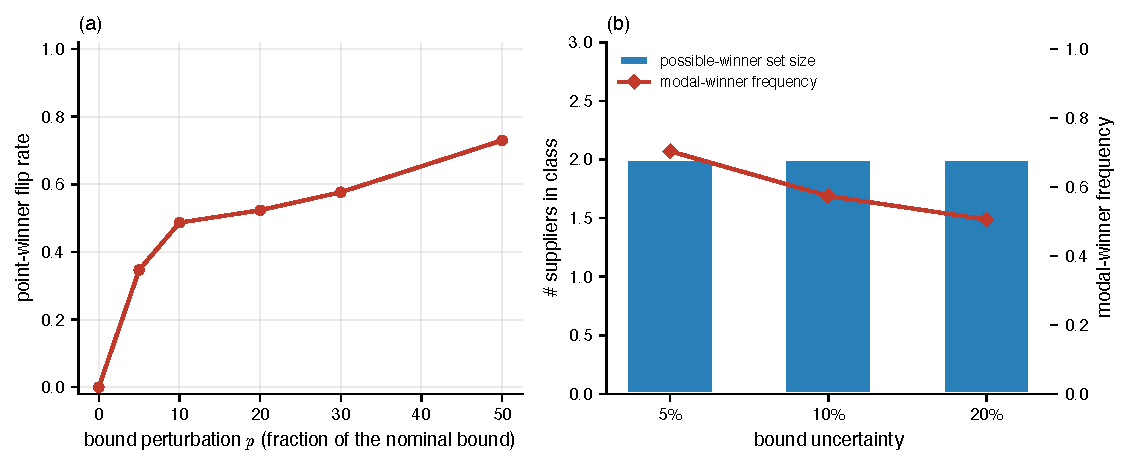
\includegraphics[width=\linewidth]{fig_supplier_interval.pdf}
\caption{Sensitivity of the fully refined ReLexTail point recommendation (black) compared to the certified possible-winner enclosures (grey) and sampled bounds (dashed) under varying uncertainty budgets for the supplier instance.}
\label{fig:interval}
\end{figure}



\section{Discussion}
\label{sec:discussion}

ReLexTail is useful when the decision maker cannot commit to precise trade-off
weights but can declare and defend a finite family of monotone scalar questions,
and when the recommendation has to be explained and re-checked afterwards. It is
not the right tool when the objective is average-case utility under a known
preference distribution, when no meaningful monotone probes can be declared or
the family is itself the political dispute, or when the bounds are so uncertain
that the possible-winner set stays large. In that last case the method still gives
the right answer, which is that the data do not support naming one alternative.

Three limitations are structural rather than fixable by more computation. The
rule depends on the candidate set, because active-set normalisation ties the
scale to the observed extremes, which dictates exactly which
edits are safe. Robustness holds relative to the declared family rather than
over all conceivable preferences, as the probe ablation shows. And the construction protects against the worst
case rather than maximising average utility, which the held-out results reflect.

Several threats to validity deserve naming. The supplier case is reproducible but synthetic; it is inspired by green supplier selection frameworks \citep{govindan2015multi, luthra2017integrated}, but constructed artificially. Validation on real decision problems is the most important
future work. The enclosures exploit affine criteria and piecewise-linear canonical probes. Nonlinear criteria or probes would require new enclosure rules. The held-out evaluation is author-chosen, restricting the hidden preferences strictly to linear losses with uniform Dirichlet weights over the criteria. The certified mode reaches only small boxes and modest criterion counts.
And the polyhedral formulation is proved for canonical probes over polyhedra
with affine criteria, with the mixed-integer branch untested and general convex
probes out of scope.

This paper introduced ReLexTail, a deterministic resolution-aware lexicographic order for auditable multicriteria selection. Under a fixed retained probe family, ReLexTail defines a complete and transitive preorder and is Pareto-compatible when the family is Pareto-separating. Its categorical prefix is stable to perturbations that do not cross category boundaries; this does not imply equivalent stability of the fully refined point recommendation. Under explicitly bounded rectangular normalisation uncertainty with positive denominators and uniformly retained probes, interval branch-and-bound yields sound possible-winner enclosures, although dependency loss may leave substantial unresolved volume. The reported empirical trade-offs apply to the tested benchmark populations and do not establish general superiority.

\section*{Declarations}

\noindent\textbf{Competing interests.} The author declares no competing
interests.

\noindent\textbf{Funding:} This research received no external funding.

\noindent\textbf{Ethics approval.} Not applicable. The study uses no human
participants, no animal subjects and no personal data.

\noindent\textbf{Data and code availability.} All data, code and seeds are in
the reproduction archive cited below. The supplier instance is constructed and
is distributed with the archive. No third-party or proprietary data is used.

\noindent\textbf{Relationship to a previous preprint.} An earlier and longer
version of this work was deposited as a preprint (Zenodo record 21037960). The
present paper supersedes it. Two classes of claim made there are withdrawn
rather than restated: an ``auditability trilemma'' framing, and the stronger
axiomatic reading of the profile-order result, which is a representation lemma
relative to a declared family and not a derivation of the leximax order from
primitive postulates. The empirical claims have also been narrowed, as
Table~\ref{tab:claims} records.

\noindent\textbf{Use of large language models.} A large language model was used
as a writing aid: to shorten prose, to check the reported numbers against the
archived outputs, and to draft regression tests. It was not used to generate
results or to design experiments. Every quantity here is computed by the
archived scripts, and the author is responsible for the whole content.

\section*{Reproducibility}

All code, data, seeds and scripts are in the archive \citep{bezoui2026archive},
version~\ArchiveVersion, at
\url{https://doi.org/10.5281/zenodo.21739625} and tagged \ArchiveRelease{} at
\url{https://github.com/MadBezoui/ReLexTail}. One command,
\texttt{python scripts/reproduce\_all.py}, regenerates every number and figure
here from the fixed master seeds. The archive also holds the full proofs, the
algorithm listings with their enclosure formulas, the per-row output of
Table~\ref{tab:truth}, the two supplier witness vectors and the audit
records.

% --- End inline part2 ---

% --- End inline body ---

\bibliography{refs}

\end{document}
